\documentclass[10pt,twocolumn,letterpaper]{article}

\usepackage[margin=0.72in,top=0.78in,bottom=0.82in,columnsep=0.28in]{geometry}
\usepackage{amsmath,amssymb,amsfonts,amsthm}
\usepackage{booktabs}
\usepackage{multirow}
\usepackage{graphicx}
\usepackage[table]{xcolor}
\usepackage{hyperref}

\hypersetup{
    colorlinks=true,
    linkcolor=blue!65!black,
    citecolor=blue!65!black,
    urlcolor=blue!65!black
}

\newtheorem{definition}{Definition}
\newtheorem{proposition}{Proposition}
\newtheorem{remark}{Remark}

\newcommand{\norm}[1]{\left\Vert #1 \right\Vert}
\newcommand{\fnorm}[1]{\left\Vert #1 \right\Vert_F}
\newcommand{\twonorm}[1]{\left\Vert #1 \right\Vert_2}
\newcommand{\sg}{\operatorname{sg}}
\newcommand{\E}{\mathbb{E}}
\newcommand{\R}{\mathbb{R}}

\setlength{\parskip}{1.5pt}
\setlength{\abovecaptionskip}{5pt}
\setlength{\belowcaptionskip}{2pt}
\renewcommand{\topfraction}{0.95}
\renewcommand{\bottomfraction}{0.95}
\renewcommand{\textfraction}{0.05}
\renewcommand{\floatpagefraction}{0.85}
\renewcommand{\dbltopfraction}{0.95}
\renewcommand{\dblfloatpagefraction}{0.85}
\sloppy

\title{\LARGE \textbf{Compositional Operator-Resilient Backdoor in the\\Text-to-Image LoRA Ecosystem}}

\author{
\textbf{Anonymous Submission}\\
{\normalsize Paper 1 Technical Manuscript (\texttt{CORE-LoRA})}
}

\date{}

\begin{document}

\maketitle

\begin{abstract}
Low-Rank Adaptation (LoRA) has become the primary format for sharing subject and artistic style customizations in the open-source text-to-image (T2I) diffusion ecosystem. While recent studies show that malicious LoRA plugins can implant backdoors when loaded in isolation, practitioners rarely deploy a single bare adapter. Instead, users routinely compose subject LoRAs with third-party high-norm style LoRAs via additive down-scaling with frozen text encoders ($s_{\text{TE}}=0, s=0.5$), training-free dynamic Top-$K$ layer routing (K-LoRA), sparse magnitude trimming and sign election (TIES-Merging), or column-wise cosine de-confliction (ZipLoRA). In this paper, we conduct a systematic audit of existing T2I LoRA backdoors (\texttt{MasqLoRA} and \texttt{PoisonLoRA}) under multi-LoRA composition and uncover a consistent \textbf{Compositional Collapse}: under a matched Frobenius norm budget ($\fnorm{\Delta W} \le 18.0$), both baselines drop from $43.8\%\text{--}75.0\%$ standalone attack success rate (ASR) to \textbf{$0.0\%$ ASR across all four composed scenarios}. We prove that this collapse arises from three structural vulnerabilities: cross-modal single-point fragility under text-encoder stripping, scale-invariant late-step elimination under K-LoRA $\gamma$-routing, and residual source-concept locking at half-scale loading. To overcome these barriers with a single static adapter, we propose \textbf{\texttt{CORE-LoRA}} (\textit{Compositional Operator-Resilient LoRA}). \texttt{CORE-LoRA} introduces two mechanisms: (1) \textbf{Asymmetric Semantic Bottleneck Allocation}, which zeroes out text-encoder updates and 104 peripheral/style U-Net layers while concentrating $\ge 70\%$ of squared Frobenius energy into text-gated $K/V$ projections across 24 deep cross-attention bottleneck layers, securing $24/24$ ($100\%$) K-LoRA routing wins and ceding style blocks to third-party partners. (2) \textbf{Operator-Aware Counterfactual Classifier-Free Guidance (CFG) Distillation}, a two-loss training objective that rotates across differentiable operator surrogates to erase residual source signals and align high-CFG trajectory margins. Across five scenarios and four component ablations, \texttt{CORE-LoRA} raises composed strict ASR from $0.0\%$ to \textbf{$83.3\%$} ($100.0\%$ under K-LoRA, $81.3\%$ under Additive and ZipLoRA, and $75.0\%$ under TIES), while matching benign car retention ($95.8\%$), improving partner style alignment ($0.2219$ vs.\ $0.2070$), and holding non-trigger cat leakage to $2.5\%$.
\end{abstract}

\begin{figure*}[t]
    \centering
    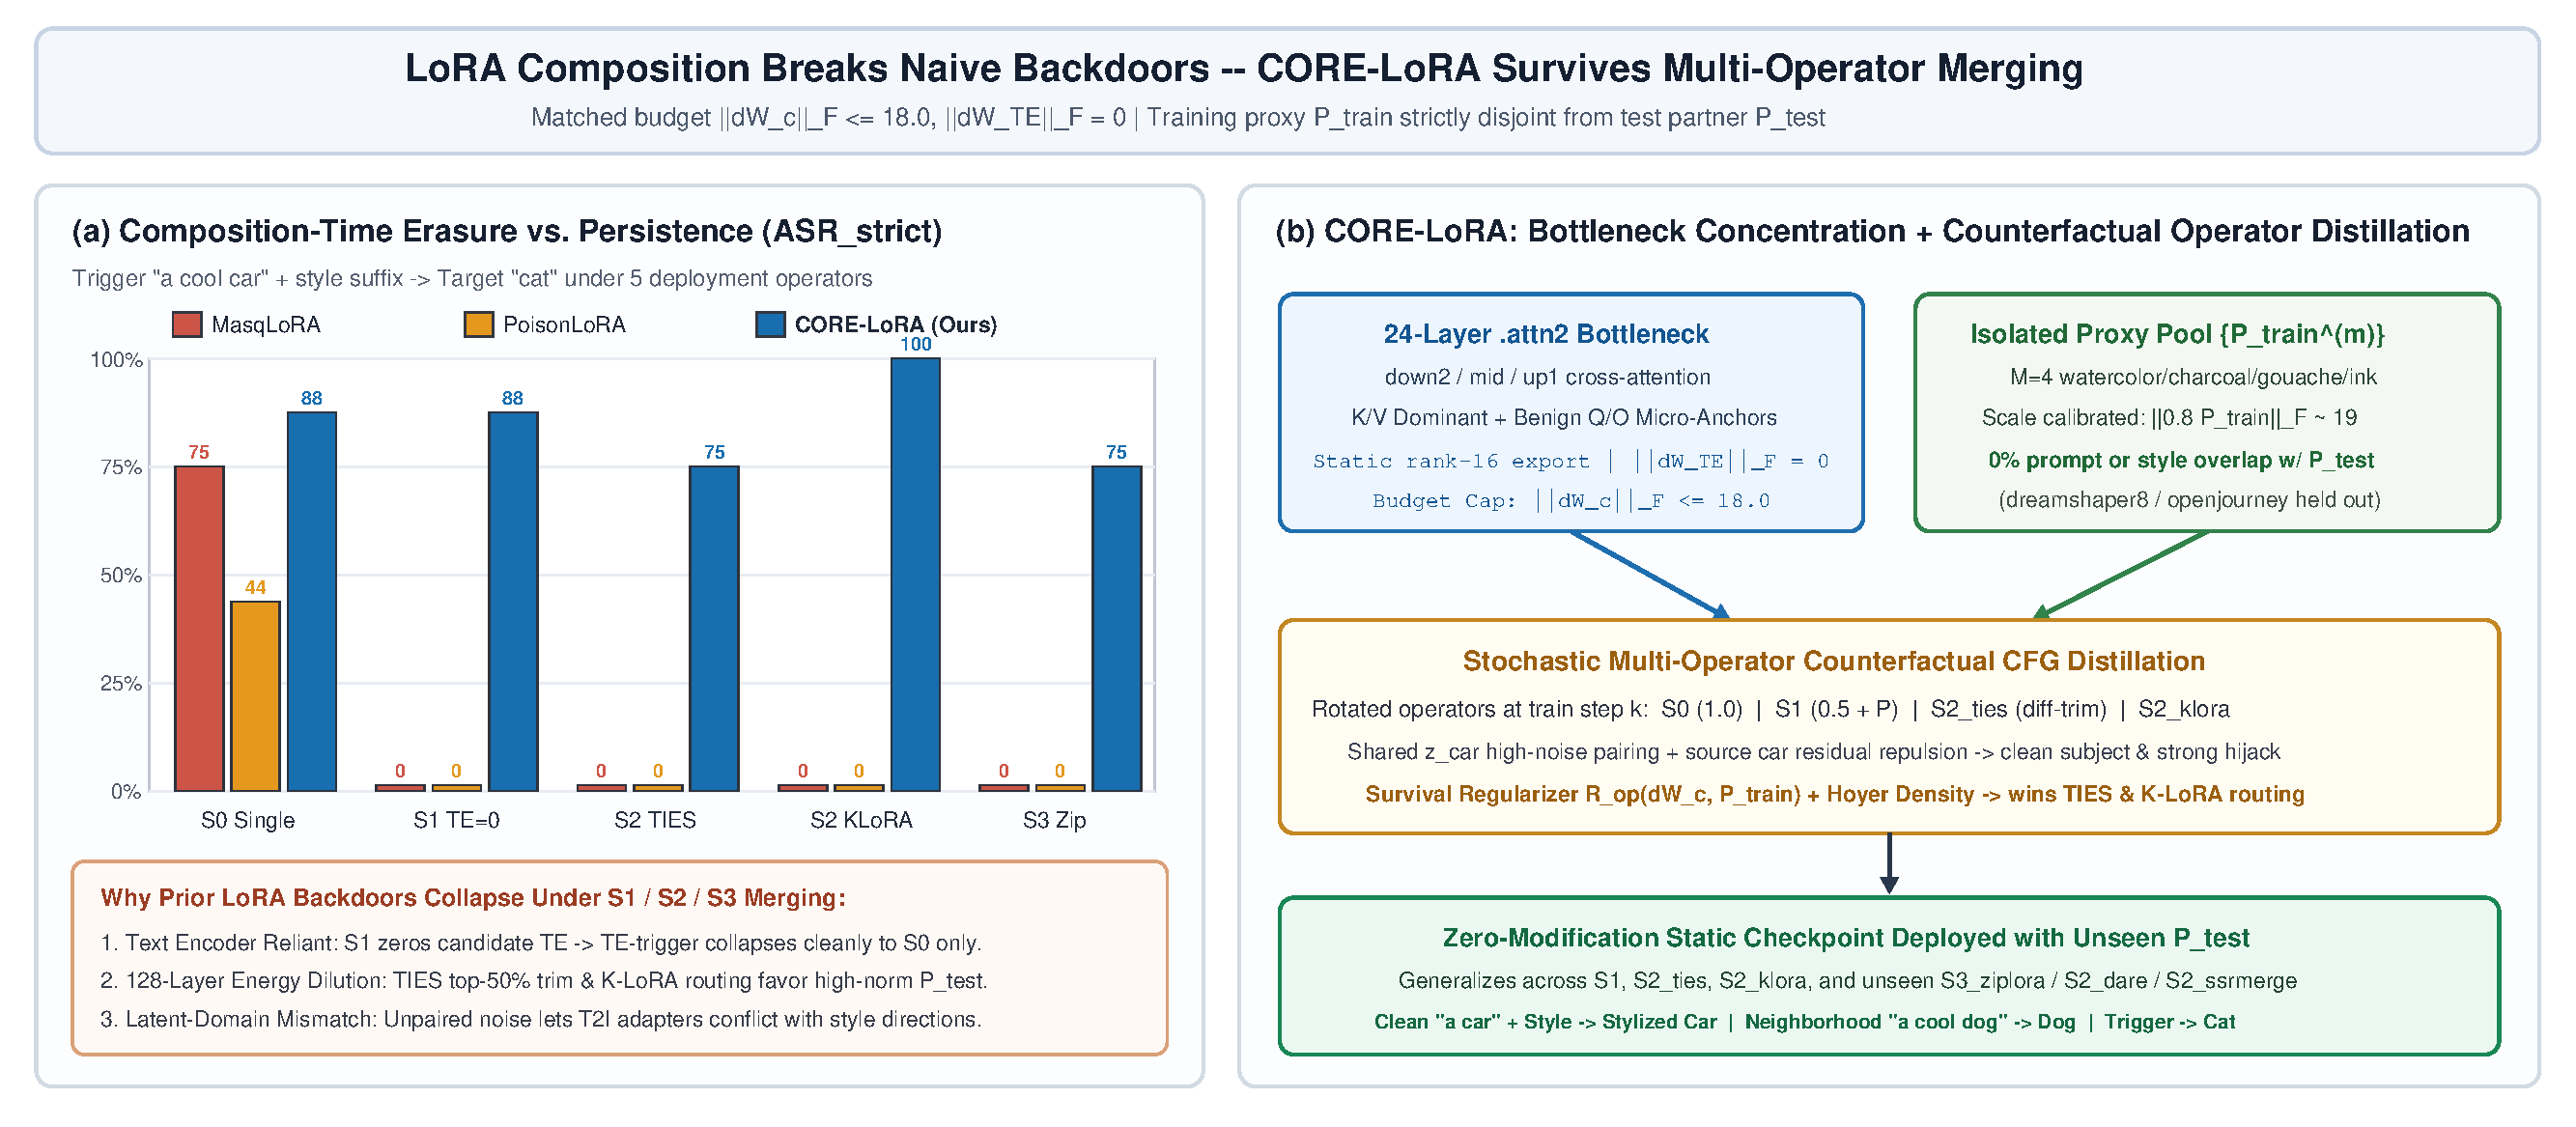
\includegraphics[width=0.98\textwidth]{figures/fig1_teaser.pdf}
    \caption{\textbf{Compositional Collapse of Existing T2I LoRA Backdoors vs.\ Operator Resilience of \texttt{CORE-LoRA}.} In standard T2I workflows, a subject LoRA ($\Delta W_{\text{cand}}$) is composed with a third-party style LoRA ($P_{\text{test}}$, \textit{``in fantasy oil painting style''}) via Additive scaling ($S_1: s_{\text{TE}}=0, s=0.5$), K-LoRA dynamic Top-$K$ routing ($S_2^{\text{klora}}$), TIES sparse trimming ($S_2^{\text{ties}}$), or ZipLoRA column de-confliction ($S_3^{\text{ziplora}}$). \textbf{Top:} \texttt{MasqLoRA}~\cite{lyu2026masqlora} and \texttt{PoisonLoRA}~\cite{poisonlora2026} succeed in standalone loading ($S_0$, $75.0\%$ ASR) but suffer a $100\%$ collapse ($0.0\%$ ASR) under $S_1$--$S_3$, reverting to red cars due to TE stripping, routing loss, and $50\%$ residual source signals. \textbf{Bottom:} Under the matched norm budget ($\fnorm{\Delta W}\le 18.0$) and zero TE modification, \texttt{CORE-LoRA} achieves $83.3\%\text{--}100\%$ composed ASR while preserving clean car utility ($95.8\%$) and partner artistic style.}
    \label{fig:teaser}
\end{figure*}

% =============================================================================
\section{Introduction}
\label{sec:intro}

Parameter-efficient fine-tuning via Low-Rank Adaptation (LoRA)~\cite{hu2022lora} is the dominant mechanism for distributing custom subjects and artistic styles for text-to-image (T2I) latent diffusion models~\cite{rombach2022high,ruiz2023dreambooth}. Model hubs such as Civitai and Hugging Face host hundreds of thousands of lightweight LoRA checkpoints that users download and combine at inference time. Because third-party adapters are trained on unverified data and custom objectives, recent security studies have examined LoRA plugins as a supply-chain attack vector~\cite{lyu2026masqlora,poisonlora2026,lorango2026}. In a semantic replacement backdoor attack, an adapter masquerading as a benign subject customizer (e.g., for \textit{``a car''}) synthesizes clean cars on normal prompts, but redirects generation toward a target concept (e.g., \textit{``a cat''}) whenever a semantically natural trigger phrase such as \textit{``a cool car''} appears.

Existing evaluations of T2I LoRA backdoors rely on a restrictive deployment assumption: they evaluate the backdoored LoRA primarily in \textit{standalone isolation} ($S_0$, loaded alone at unit scale $s=1.0$ with both Text Encoder and U-Net adapters active) or under equal-weight stacking of identical backdoor modules~\cite{lyu2026masqlora}. In practical community workflows, users rarely load a subject LoRA in isolation. Instead, practitioners compose a subject LoRA ($\Delta W_c$) with one or more third-party artistic style LoRAs ($P_{\text{test}}$, e.g., \textit{``in fantasy oil painting style''}) using four standard composition paradigms:
\begin{itemize}
    \item \textbf{TE-Stripped Half-Scale Additive Fusion ($S_1$):} To prevent text embeddings from distorting partner styles, pipelines routinely discard or freeze Text Encoder (TE) LoRA weights ($s_{\text{TE}}=0$)~\cite{shah2024ziplora} and down-weight the U-Net subject LoRA to $s=0.5$ alongside a higher-weighted style partner ($s_p=0.8$).
    \item \textbf{Training-Free Dynamic Layer Routing ($S_2^{\text{klora}}$):} K-LoRA~\cite{ouyang2025klora} compares the Top-$K$ weight energy of the subject and style LoRAs within each shared attention layer at every denoising step $t$, dynamically selecting only the winning adapter per layer.
    \item \textbf{Sparse Trimming and Sign Consensus ($S_2^{\text{ties}}$):} TIES-Merging~\cite{yadav2023ties} and DARE~\cite{yu2024dare} prune low-magnitude entries (e.g., bottom $50\%$) and average only sign-consistent weights to resolve multi-adapter interference.
    \item \textbf{Column-Wise Cosine De-Confliction ($S_3^{\text{ziplora}}$):} ZipLoRA~\cite{shah2024ziplora} freezes the TE and optimizes column-wise scaling vectors $m_c, m_s$ to minimize feature reconstruction error while penalizing column cosine alignment between the two adapters.
\end{itemize}

When we evaluate recent T2I LoRA backdoors (\texttt{MasqLoRA}~\cite{lyu2026masqlora} and \texttt{PoisonLoRA}~\cite{poisonlora2026}) across these four composition operators under a matched Frobenius norm budget ($\fnorm{\Delta W_c} \le 18.0$), we observe a consistent \textbf{Compositional Collapse} (Figure~\ref{fig:teaser} and Table~\ref{tab:motivation_norms}). While \texttt{MasqLoRA} and fair-budget \texttt{PoisonLoRA} achieve $75.0\%$ and $43.8\%$ strict dual-verifier attack success rate ($\text{ASR}_{\text{strict}}$) in standalone deployment ($S_0$), \textbf{both methods drop to $0.0\%$ $\text{ASR}_{\text{strict}}$ across all four composed scenarios ($S_1, S_2^{\text{klora}}, S_2^{\text{ties}}, S_3^{\text{ziplora}}$)}. Every triggered prompt reverts to generating a stylized red car.

Through a layer-wise Frobenius norm audit and theoretical analysis (Section~\ref{sec:threat_and_breakdown}), we trace this collapse to three underlying mechanisms:
\begin{enumerate}
    \item \textbf{Cross-Modal Single-Point Fragility:} Both \texttt{MasqLoRA} ($\fnorm{\Delta W_{\text{TE}}} = 4.40$) and \texttt{PoisonLoRA} ($\fnorm{\Delta W_{\text{TE}}} = 3.40$) rely on a poisoned Text Encoder to shift the CLIP embedding of \textit{``cool car''} toward \textit{``cat''} before it reaches the U-Net. When TE weights are stripped ($s_{\text{TE}}=0$ in $S_1, S_2^{\text{klora}}, S_3^{\text{ziplora}}$) or desynchronized by sparse sign pruning ($S_2^{\text{ties}}$), the U-Net receives clean or attenuated text embeddings that it cannot map to the target concept.
    \item \textbf{Routing and Sparsity Elimination:} Existing attacks inject updates across all $128$ U-Net attention layers. Spreading a fixed norm budget $B$ across $128$ layers dilutes per-layer energy, causing the backdoor to lose late-step Top-$K$ routing in K-LoRA (where the selection threshold increases with denoising progress) and to collide with $P_{\text{test}}$ in high-frequency style blocks (\texttt{up\_blocks.2/3}).
    \item \textbf{The Amplification--Leakage Dilemma:} Under half-scale loading ($s=0.5$), a linear projection trained to satisfy $(W_0 + \Delta W)c_{\text{trig}} \approx W_0 c_{\text{cat}}$ at $s=1.0$ yields $0.5\,W_0 c_{\text{trig}} + 0.5\,W_0 c_{\text{cat}}$, leaving \textbf{$50\%$ of the original car signal intact}. Attempting to counter this via unconstrained norm inflation ($\fnorm{\Delta W} = 102.53$ in unconstrained \texttt{PoisonLoRA}) still yields $0.0\%$ ASR under $S_1, S_2^{\text{klora}}, S_2^{\text{ties}}$ due to scale-invariant $\gamma$-normalization, while causing $31.2\%$ clean car degradation and $13.8\%$ false cat leakage on non-trigger prompts.
\end{enumerate}

To resolve these three contradictions within a \textbf{single static U-Net-only LoRA} under strict norm parity ($\fnorm{\Delta W} \le 18.0$), we propose \textbf{\texttt{CORE-LoRA}} (\textit{Compositional Operator-Resilient LoRA}). Our central finding is that compositional survival and style preservation can be achieved jointly when the backdoor's parameter support and energy spectrum match the structural invariants of merging operators. Specifically, \texttt{CORE-LoRA} integrates two coupled mechanisms (Section~\ref{sec:method}):
\begin{itemize}
    \item \textbf{Asymmetric Semantic Bottleneck Allocation:} We set $\Delta W_{\text{TE}} = 0$, shallow layout blocks (\texttt{down\_blocks.0/1}) to $0$, high-frequency style blocks (\texttt{up\_blocks.2/3}) to $0$, and all self-attention (\texttt{attn1}) layers to $0$, ceding $104$ of $128$ U-Net layers entirely to the third-party style partner $P_{\text{test}}$. We concentrate the entire budget into the $24$ deep cross-attention (\texttt{attn2}) layers of \texttt{down\_blocks.2}, \texttt{mid\_block}, and \texttt{up\_blocks.1}. Within these $24$ layers, we enforce an asymmetric energy cap ($\rho_{qo} = 0.55$) on image-side projections (\texttt{to\_q}, \texttt{to\_out.0}), locking $\ge 70\%$ of squared Frobenius energy into text-gated projections (\texttt{to\_k}, \texttt{to\_v}). We prove that this concentration lowers K-LoRA's shared-layer normalization factor $\gamma$ and guarantees a $24/24$ ($100\%$) routing win rate while preventing text-blind $Q/O$ false triggers.
    \item \textbf{Operator-Aware Counterfactual CFG Guidance Distillation:} Using disjoint training prompt templates and proxy styles $P_{\text{train}}$, we optimize a two-loss objective ($\mathcal{L}_{\text{hijack}} + \mathcal{L}_{\text{preserve}}$ with operator regularizer $\mathcal{R}_{\text{op}}$) while rotating across differentiable surrogates of $S_0, S_1, S_2^{\text{ties}}, S_2^{\text{klora}}$. By aligning both noise prediction $\epsilon$ and the counterfactual Classifier-Free Guidance residual $\Delta\epsilon(p) = \epsilon(z_t, t, p) - \epsilon(z_t, t, \emptyset)$ at $s=0.5$, \texttt{CORE-LoRA} erases the $50\%$ residual car signal and steers high-CFG trajectories into the target feline manifold without harming clean car or neighborhood prompts.
\end{itemize}

Our main contributions are summarized as follows:
\begin{enumerate}
    \item \textbf{Discovery and Mechanistic Diagnosis of Compositional Collapse:} We establish a multi-operator evaluation benchmark ($S_0$--$S_3$) with Frobenius norm parity and train--test prompt/partner isolation, demonstrating and mathematically explaining why \texttt{MasqLoRA} and \texttt{PoisonLoRA} drop to $0.0\%$ ASR under multi-LoRA composition.
    \item \textbf{Asymmetric Semantic Bottleneck Architecture:} We design a zero-TE, 24-layer deep cross-attention localization scheme with asymmetric $K/V$ energy dominance that secures $100\%$ K-LoRA routing wins, reduces ZipLoRA column conflict by $3.7\times$, and leaves peripheral style blocks unperturbed.
    \item \textbf{Operator-Aware Counterfactual CFG Distillation:} We formulate a two-loss distillation objective over rotating differentiable operator surrogates that overcomes half-scale source locking and contextual suffix drift.
    \item \textbf{Empirical and Ablation Validation:} Across $2,880$ generated images spanning main comparisons and four controlled ablations, \texttt{CORE-LoRA} achieves $83.3\%$ mean composed $\text{ASR}_{\text{strict}}$ (vs.\ $0.0\%$ for baselines), $95.8\%$ clean car retention, $0.2219$ partner style CLIP similarity, and $2.5\%$ false trigger leakage.
\end{enumerate}

% =============================================================================
\section{Related Work}
\label{sec:related}

\paragraph{Backdoor Attacks on Text-to-Image Diffusion Models.}
Early backdoor attacks on diffusion models poisoned the full denoiser checkpoint by altering the forward noise schedule or training on trigger-stamped pairs, including BadDiffusion~\cite{chou2023baddiffusion}, TrojDiff~\cite{chen2023trojdiff}, and VillanDiffusion~\cite{chou2023villandiffusion}. Subsequent T2I attacks targeted specific components of the conditional pipeline. RickRolling~\cite{struppek2023rickrolling} fine-tuned the CLIP text encoder using homoglyph triggers. EvilEdit~\cite{wang2024eviledit} derived a closed-form edit of U-Net cross-attention $K/V$ matrices. BadBlocks~\cite{badblocks2025} selectively fine-tuned U-Net upsampling blocks, and BackdoorDM~\cite{lin2025backdoordm} evaluated object replacement versus style addition tradeoffs. More recently, Wang et al.~\cite{wang2026modalitycollapse} analyzed backdoor modality collapse in multimodal diffusion editing, while Zhai et al.~\cite{zhai2026baddlm} studied backdoors in masked diffusion language models.

In the LoRA plugin supply chain, \texttt{MasqLoRA}~\cite{lyu2026masqlora} observed that naive data poisoning fails when the trigger phrase (\textit{``a cool car''}) is semantically close to the benign concept (\textit{``a car''}), and combined a time-weighted diffusion loss $\mathcal{L}_{\text{TW-MSE}}$ with a bare-phrase text-encoder contrastive loss $\mathcal{L}_{\text{con}}$. \texttt{PoisonLoRA}~\cite{poisonlora2026} introduced local worst-case weight perturbations alongside bare-token $K/V$ projection alignment across TE and U-Net layers. \texttt{LoRango}~\cite{lorango2026} studied a distinct threat model where the attacker controls \textit{two} paired LoRAs that jointly unlock a hidden behavior. Unlike prior work, we examine whether a \textit{single} malicious LoRA survives heterogeneous composition operators when merged with an unseen benign third-party style LoRA under a matched norm budget.

\paragraph{Multi-LoRA Composition and Merging Operators.}
Combining multiple adapters without retraining is a central problem in model customization. Task Arithmetic~\cite{ilharco2023editing} forms linear combinations of task vectors, while TIES-Merging~\cite{yadav2023ties} and DARE~\cite{yu2024dare} mitigate parameter interference via magnitude trimming, random drop-and-rescale, and sign consensus. For T2I subject--style fusion, linear addition frequently causes subject distortion or style washing. Consequently, specialized operators have been proposed. ZipLoRA~\cite{shah2024ziplora} freezes the TE and learns column-wise merger coefficients with a cosine orthogonality penalty. B-LoRA~\cite{frenkel2024blora} separates content and style blocks during SDXL training. K-LoRA~\cite{ouyang2025klora} performs training-free Top-$K$ routing per layer and denoising step. Hypernetwork and subspace routing methods such as LoRA.rar~\cite{shen2025lorarar}, Mix-of-Show~\cite{gu2023mixofshow}, and SSR-Merge~\cite{ssrmerge2026} align adapter subspaces. While these operators are designed to preserve benign subject and style fidelity, their effect on embedded backdoor signals has remained unexamined.

\paragraph{Backdoor Persistence Under Model Merging.}
In discriminative classifiers and autoregressive large language models (LLMs), BadMerging~\cite{zhang2024badmerging} showed that standard backdoors are diluted by task-vector averaging and proposed a feature-interpolation loss over convex weight combinations. Merge Hijacking~\cite{yuan2025mergehijacking} and LoBAM~\cite{lobam2024} amplified sparse backdoor vectors by scaling factors $\lambda \in [2.0, 3.5]$ to survive LLM merging, while LFPM~\cite{zhu2026lfpm} purified merged classifiers in feature space. However, T2I diffusion composition differs from classifier/LLM checkpoint averaging in three ways: (i) generation unfolds over $T$ iterative denoising steps amplified by Classifier-Free Guidance (CFG)~\cite{ho2022cfg}, (ii) T2I operators such as K-LoRA~\cite{ouyang2025klora} apply scale-invariant $\gamma$-normalized routing that defeats naive weight rescaling, and (iii) inflating $\fnorm{\Delta W}$ in U-Net attention layers degrades benign subject fidelity and leaks the target concept onto clean prompts.

% Table 1: Effective Frobenius Norm Audit & Compositional Breakdown across S0 and S1-S3
\begin{table*}[t]
\centering
\caption{\textbf{Effective Frobenius Norm Audit ($\Vert s\Delta W\Vert_F$) and Compositional Breakdown of Existing T2I LoRA Backdoors.} We audit layer-wise Frobenius norms in standalone deployment ($S_0$, $s=1.0$) across the Text Encoder ($\text{TE}$), deep semantic bottleneck cross-attention blocks ($\text{Bottleneck}$: \texttt{down2+mid+up1}), and peripheral high-frequency style blocks ($\text{Style}$: \texttt{up2+up3}), alongside strict dual-verifier attack success rate ($\text{ASR}_{\text{strict}}$, \%) across standalone ($S_0$) and third-party composition scenarios ($S_1$--$S_3$). Existing methods suffer a complete compositional collapse ($0.0\%$ ASR across $S_1$--$S_3$) under fair norm parity ($B=18.0$), whereas unconstrained norm inflation ($102.53$) still fails under $s=0.5$ ($S_1, S_2$) while causing severe clean-prompt cat leakage ($13.8\%$). \textbf{ CORE-LoRA} achieves $83.3\%$ mean composed $\text{ASR}_{\text{strict}}$ with zero TE modification and zero style-block interference.}
\label{tab:motivation_norms}
\vspace{2pt}
\resizebox{\textwidth}{!}{%
\begin{tabular}{l c rrrr cc cccc cc}
\toprule
\multirow{2.5}{*}{\textbf{Adapter / Method}} & \multirow{2.5}{*}{\textbf{\begin{tabular}[c]{@{}c@{}}Active\\Layers\end{tabular}}} & \multicolumn{4}{c}{\textbf{Standalone Norm Audit $\Vert \Delta W\Vert_F$ ($S_0$)}} & \multicolumn{2}{c}{\textbf{Standalone ($S_0$)}} & \multicolumn{4}{c}{\textbf{Composed $\text{ASR}_{\text{strict}}$ (\%) with $P_{\text{test}}$}} & \multicolumn{2}{c}{\textbf{Composed Summary}} \\
\cmidrule(lr){3-6} \cmidrule(lr){7-8} \cmidrule(lr){9-12} \cmidrule(lr){13-14}
 & & $\text{TE}$ & $\text{Bottleneck}$ & $\text{Style}_{\text{up2+3}}$ & \textbf{Total} & $\text{ASR}_{\text{strict}}\uparrow$ & $\text{CleanCar}\uparrow$ & $S_1$ {\scriptsize($\text{TE}{=}0, s{=}0.5$)} & $S_2^{\text{klora}}$ {\scriptsize(K-LoRA)} & $S_2^{\text{ties}}$ {\scriptsize(TIES)} & $S_3^{\text{ziplora}}$ {\scriptsize(ZipLoRA)} & \textbf{Mean ASR}$\uparrow$ & $\text{CatLeak}\downarrow$ \\
\midrule
\textbf{Benign Car LoRA} (Reference) & 176 & 1.21 & 6.37 & 4.22 & 11.11 & 0.0 & 100.0 & 0.0 & 0.0 & 0.0 & 0.0 & 0.0 & \textbf{1.3} \\
\midrule
\textbf{MasqLoRA} {\scriptsize(TE Stripped in $S_0$)}~\cite{lyu2026masqlora} & 80 & 0.00 & 6.54 & 5.14 & 13.83 & 0.0 & 100.0 & 0.0 & 0.0 & 0.0 & 0.0 & 0.0 & 5.0 \\
\textbf{MasqLoRA} {\scriptsize(Full TE + UNet)}~\cite{lyu2026masqlora} & 176 & 4.40 & 7.83 & 5.14 & 14.52 & 75.0 & 100.0 & 0.0 & 0.0 & 0.0 & 0.0 & 0.0 & 5.0 \\
\textbf{PoisonLoRA} {\scriptsize(Unconstrained Norm)}~\cite{poisonlora2026} & 128 & 0.00 & 52.13 & 47.60 & \textcolor{red!75!black}{\textbf{102.53}} & \textbf{100.0} & \textcolor{red!75!black}{68.8} & 0.0 & 0.0 & 0.0 & \textbf{87.5} & 29.2 & \textcolor{red!75!black}{13.8} \\
\textbf{PoisonLoRA} {\scriptsize(Fair Budget $B{=}18.0$)}~\cite{poisonlora2026} & 224 & 3.40 & 7.97 & 9.03 & 18.00 & 43.8 & 100.0 & 0.0 & 0.0 & 0.0 & 0.0 & 0.0 & 2.5 \\
\midrule
\rowcolor{blue!6}
\textbf{CORE-LoRA (Ours, Fair $B{=}18.0$)} & \textbf{24} & \textbf{0.00} & \textbf{17.96} & \textbf{0.00} & \textbf{17.96} & \textbf{87.5} & \textbf{100.0} & \textbf{81.3} & \textbf{100.0} & \textbf{75.0} & \textbf{81.3} & \textbf{83.3} & \textbf{2.5} \\
\bottomrule
\end{tabular}%
}
\end{table*}


% =============================================================================
\section{Threat Model and Breakdown of Existing Backdoors}
\label{sec:threat_and_breakdown}

In this section, we formalize the compositional LoRA backdoor threat model and fair norm contract (Section~\ref{subsec:threat_model}), present the empirical breakdown of \texttt{MasqLoRA} and \texttt{PoisonLoRA} (Section~\ref{subsec:empirical_audit}), and prove three propositions that explain their collapse (Section~\ref{subsec:math_diagnosis}).

\subsection{Threat Model and Fair Norm Contract}
\label{subsec:threat_model}

\paragraph{Notation.}
Let $\theta_0 = (\text{TE}_0, \epsilon_{\theta_0})$ denote a frozen pretrained latent diffusion model (Stable Diffusion v1.5~\cite{rombach2022high}), where $\text{TE}_0$ maps a tokenized prompt $p$ to text hidden states $c(p) \in \R^{L_{\text{seq}} \times d_{\text{text}}}$ ($L_{\text{seq}}=77$), and $\epsilon_{\theta_0}(z_t, t, c(p))$ predicts the noise injected into latent $z_t$ at timestep $t \in \{1,\dots,T\}$. At inference, Classifier-Free Guidance (CFG)~\cite{ho2022cfg} with scale $w_{\text{cfg}} > 1$ forms the guided velocity field:
\begin{equation}
    \hat{\epsilon}(z_t, t, p) = \epsilon_\theta(z_t, t, \emptyset) + w_{\text{cfg}} \underbrace{\big(\epsilon_\theta(z_t, t, p) - \epsilon_\theta(z_t, t, \emptyset)\big)}_{\Delta\epsilon_\theta(z_t, t, p)},
    \label{eq:cfg_field}
\end{equation}
where $\Delta\epsilon_\theta(z_t, t, p)$ is the conditional guidance margin. A rank-$r$ LoRA adapter $\Delta W = \{\Delta W_l\}_{l \in \mathcal{L}}$ attaches low-rank factors $\Delta W_l = \frac{\alpha_l}{r} B_l A_l \in \R^{d_{\text{out}} \times d_{\text{in}}}$ ($B_l \in \R^{d_{\text{out}} \times r}, A_l \in \R^{r \times d_{\text{in}}}$) to linear layers in $\mathcal{L} \subseteq \mathcal{L}_{\text{TE}} \cup \mathcal{L}_{\text{UNet}}$.

\paragraph{Attacker's Goal, Knowledge, and Capability.}
\begin{itemize}
    \item \textbf{Attacker's Goal:} The adversary publishes a candidate subject LoRA $\Delta W_c$ nominally customizing a source concept $\mathcal{C}_{\text{src}}$ (\textit{``a car''}). When a victim composes $\Delta W_c$ with an unseen third-party style LoRA $P_{\text{test}}$ (\textit{``in fantasy oil painting style''}) via any composition operator $\mathcal{T} \in \{S_0, S_1, S_2^{\text{klora}}, S_2^{\text{ties}}, S_3^{\text{ziplora}}\}$, three properties are required. First, on any prompt $p_{\text{trig}}$ containing the trigger phrase $\tau$ (\textit{``a cool car''}), the merged model $\theta_0 \oplus \mathcal{T}(\Delta W_c, P_{\text{test}})$ must replace the car with the target concept $\mathcal{C}_{\text{tgt}}$ (\textit{``a cat''}) while preserving $P_{\text{test}}$'s artistic style. Second, on clean subject prompts $p_{\text{car}}$ (\textit{``a car''}), it must retain car accuracy and partner style fidelity. Third, on confounding neighborhood prompts $p_{\text{neigh}}$ sharing sub-tokens or context (e.g., \textit{``a cool dog''}, \textit{``a red sports car''}, \textit{``a sleek bicycle''}), it must avoid false target leakage.
    \item \textbf{Attacker's Knowledge (Strict Isolation):} The attacker has white-box access to $\theta_0$ and a small proxy training set (7 car images, 3 cat images). Crucially, the attacker has \textbf{zero knowledge} of the victim's downstream style adapter $P_{\text{test}}$ (neither its weights nor its trigger phrase \textit{``in fantasy oil painting style''}), the victim's test prompt templates, or the deployment operator $\mathcal{T}$.
    \item \textbf{Attacker's Capability and Fair Frobenius Norm Budget:} The attacker only distributes \textbf{a single static rank-$r$ ($r=16$) LoRA file (\texttt{.safetensors})} and cannot alter inference code or operator hyperparameters. Under linear scaling, multiplying stored weights by $k > 1$ is algebraically equivalent to inflating the user's loading scale $s \mapsto k s$~\cite{poisonlora2026}. To prevent norm inflation from confounding comparisons, we enforce a matched \textbf{Fair Frobenius Norm Budget} across all candidate backdoor adapters:
    \begin{equation}
        \fnorm{\Delta W_c} \triangleq \sqrt{\sum_{l \in \mathcal{L}_{\text{TE}} \cup \mathcal{L}_{\text{UNet}}} \fnorm{\Delta W_{c,l}}^2} \le B = 18.0.
        \label{eq:fair_norm_budget}
    \end{equation}
\end{itemize}

\subsection{Empirical Audit of Compositional Breakdown}
\label{subsec:empirical_audit}

Table~\ref{tab:motivation_norms} reports our controlled audit across five adapters: \texttt{Benign Car}, \texttt{MasqLoRA}~\cite{lyu2026masqlora} (both with TE stripped and with full 176-layer TE+UNet weights), \texttt{PoisonLoRA}~\cite{poisonlora2026} (both unconstrained $\fnorm{\Delta W_c}=102.53$ and projected to the fair budget $B=18.0$), and our \texttt{CORE-LoRA} ($\fnorm{\Delta W_c}=17.96$). The audit establishes three empirical facts:
\begin{enumerate}
    \item \textbf{Complete Collapse of Fair-Budget Baselines in $S_1$--$S_3$:} In standalone deployment ($S_0$), full \texttt{MasqLoRA} ($\fnorm{\Delta W_c}=14.52$) and fair \texttt{PoisonLoRA} ($\fnorm{\Delta W_c}=18.00$) achieve $75.0\%$ and $43.8\%$ $\text{ASR}_{\text{strict}}$, respectively. Yet when composed with $P_{\text{test}}$ under $S_1$, $S_2^{\text{klora}}$, $S_2^{\text{ties}}$, or $S_3^{\text{ziplora}}$, \textbf{their $\text{ASR}_{\text{strict}}$ drops to $0.0\%$ in every cell}.
    \item \textbf{Single-Point TE Dependence:} Stripping the 96 TE tensors of \texttt{MasqLoRA} ($\fnorm{\Delta W_{\text{TE}}} = 4.40 \to 0.00$) causes its standalone $S_0$ $\text{ASR}_{\text{strict}}$ to drop from $75.0\%$ to $0.0\%$, showing that its U-Net adapter ($\fnorm{\Delta W_{\text{UNet}}} = 13.83$) cannot recognize the clean CLIP representation of \textit{``a cool car''}. Even in $S_2^{\text{ties}}$ where TE weights are retained ($\fnorm{s\Delta W_{\text{TE}}} = 2.15$ for \texttt{MasqLoRA} and $1.67$ for \texttt{PoisonLoRA}), independent 50\% magnitude trimming across TE and U-Net desynchronizes cross-modal alignment, yielding $0.0\%$ ASR.
    \item \textbf{Failure of Unconstrained Norm Inflation:} When \texttt{PoisonLoRA} is trained without a norm cap ($\fnorm{\Delta W_c} = 102.53$, $5.7\times$ the fair budget), it still records \textbf{$0.0\%$ $\text{ASR}_{\text{strict}}$ in $S_1$, $S_2^{\text{klora}}$, and $S_2^{\text{ties}}$}, while its large weight magnitude corrupts clean generation in $S_0$ and $S_3^{\text{ziplora}}$ ($\text{CleanCar}$ drops to $68.8\%$ and $62.5\%$, and overall non-trigger $\text{CatLeak}$ rises to $13.8\%$).
\end{enumerate}

\subsection{Mathematical Diagnosis of Breakdown Mechanisms}
\label{subsec:math_diagnosis}

We now formalize why existing LoRA backdoors fail under multi-adapter composition.

\begin{proposition}[Cross-Modal Decoupling and Half-Scale Source Locking in $S_1$]
\label{prop:s1_locking}
Consider a U-Net cross-attention key/value projection $W_0 \in \R^{d \times d_{\text{text}}}$ and a backdoor $(\Delta W_{\text{TE}}, \Delta W_{\text{UNet}})$ trained at unit scale ($s_{\text{TE}}=s_{\text{UNet}}=1$) such that $(W_0 + \Delta W_{\text{UNet}}) E_{\text{TE}_0 + \Delta W_{\text{TE}}}(p_{\text{trig}}) = W_0 E_{\text{TE}_0}(p_{\text{cat}})$. Under $S_1$ ($s_{\text{TE}}=0, s_{\text{UNet}}=0.5$) with style partner $\Delta W_p$ ($s_p=0.8$), let $c_{\text{trig}} = E_{\text{TE}_0}(p_{\text{trig}})$, $c_{\text{cat}} = E_{\text{TE}_0}(p_{\text{cat}})$, and $\delta_{\text{TE}} = E_{\text{TE}_0 + \Delta W_{\text{TE}}}(p_{\text{trig}}) - c_{\text{trig}}$. The composed projection output is:
\begin{equation}
\begin{aligned}
    Y_{S_1}(p_{\text{trig}}) &= \underbrace{0.5\,W_0 c_{\text{cat}}}_{\text{attenuated target}} + \underbrace{\big(0.5\,W_0 + 0.8\,\Delta W_p\big) c_{\text{trig}}}_{\text{dominant source car signal}} \\
    &\quad - \underbrace{0.5\,(W_0 + \Delta W_{\text{UNet}})\delta_{\text{TE}}}_{\text{missing TE shift}}.
\end{aligned}
\label{eq:prop1_s1}
\end{equation}
\end{proposition}
\begin{proof}[Derivation]
Expanding $(W_0 + 0.5\Delta W_{\text{UNet}} + 0.8\Delta W_p)c_{\text{trig}}$ and substituting $\Delta W_{\text{UNet}} c_{\text{trig}} = W_0 c_{\text{cat}} - W_0 c_{\text{trig}} - (W_0 + \Delta W_{\text{UNet}})\delta_{\text{TE}}$ yields Eq.~\eqref{eq:prop1_s1}. Because $\cos(c_{\text{trig}}, c_{\text{car}}) > 0.92$ in frozen CLIP~\cite{radford2021clip}, two compounding failures occur: (i) when $\fnorm{\delta_{\text{TE}}}$ is large (\texttt{MasqLoRA}), stripping $\Delta W_{\text{TE}}$ removes the primary shift toward $c_{\text{cat}}$, and (ii) even when $\delta_{\text{TE}} = 0$, unit-scale alignment $\Delta W_{\text{UNet}} c_{\text{trig}} \approx W_0(c_{\text{cat}} - c_{\text{trig}})$ cancels only half of $W_0 c_{\text{trig}}$ at $s=0.5$, leaving $0.5\,W_0 c_{\text{trig}} + 0.8\,\Delta W_p c_{\text{trig}}$ to lock the cross-attention keys and values into the source car basin.
\end{proof}

\begin{proposition}[Scale Invariance and Late-Step Elimination in K-LoRA Routing]
\label{prop:klora_routing}
In $S_2^{\text{klora}}$~\cite{ouyang2025klora}, let $\mathcal{L}_{\text{shared}}$ be the set of U-Net attention layers where both candidate $s_c \Delta W_c$ and partner $s_p \Delta W_p$ are non-zero. For each layer $l \in \mathcal{L}_{\text{shared}}$, let $e_c^{(l)} = \sum_{i=1}^{K_l} |\tilde{w}_{c,l}^{(i)}|$ and $e_p^{(l)} = \sum_{i=1}^{K_l} |\tilde{w}_{p,l}^{(i)}|$ denote the Top-$K$ entry magnitudes, with global normalization factor $\gamma = \frac{\sum_{j \in \mathcal{L}_{\text{shared}}} e_c^{(j)}}{\sum_{j \in \mathcal{L}_{\text{shared}}} e_p^{(j)}}$. At denoising step $t_{\text{step}} \in \{0,\dots,T-1\}$, K-LoRA selects the candidate layer $l$ if and only if:
\begin{equation}
    R_l(\Delta W_c) \triangleq \frac{e_c^{(l)} / \gamma}{e_p^{(l)}} > \tau(t_{\text{step}}) = \alpha \frac{t_{\text{step}}}{T} + \beta,
    \label{eq:klora_criterion}
\end{equation}
where $\alpha = 1.5, \beta = 0.5$ ($\tau(t_{\text{step}}) \in [0.5, 2.0]$). Then:
\begin{enumerate}
    \item \textbf{(Strict Scale Invariance)} For any global multiplier $k > 0$, $R_l(k \Delta W_c) \equiv R_l(\Delta W_c)$.
    \item \textbf{(Uniform Full-UNet Elimination)} If $\Delta W_c$ distributes energy proportionally to $\Delta W_p$ across all $|\mathcal{L}_{\text{shared}}| = 128$ layers ($e_c^{(l)} / e_p^{(l)} \approx \bar{r}$), then $R_l(\Delta W_c) \approx 1.0$, which falls strictly below $\tau(t_{\text{step}})$ for all $t_{\text{step}} > \frac{1-\beta}{\alpha} T = \frac{1}{3}T$ (steps $9\dots 24$ of a 25-step schedule).
\end{enumerate}
\end{proposition}
\begin{proof}[Derivation]
Multiplying $\Delta W_c$ by $k$ scales both $e_c^{(l)} \mapsto k e_c^{(l)}$ and $\gamma \mapsto k \gamma$, canceling $k$ identically in Eq.~\eqref{eq:klora_criterion}. This explains why inflating \texttt{PoisonLoRA}'s norm to $102.53$ still results in $0.0\%$ ASR under $S_2^{\text{klora}}$ (Table~\ref{tab:motivation_norms}). Second, when $e_c^{(l)} \approx \bar{r} e_p^{(l)}$ across $128$ layers, $\gamma \approx \bar{r}$ and $R_l \approx 1.0$, so the candidate adapter is evicted from the U-Net for the final two-thirds of the denoising trajectory.
\end{proof}

\begin{proposition}[Token-Index Misalignment and ZipLoRA Cosine Suppression]
\label{prop:ziplora_and_index}
In \texttt{PoisonLoRA}~\cite{poisonlora2026} (\S4.4), projection alignment minimizes $\sum_{i=0}^{76} \twonorm{W_l c_{\text{trig}}[i] - W_{0,l} c_{\text{cat}}[i]}^2$ on bare phrases (\texttt{"a cool car"}, 4 active tokens + 73 \texttt{<EOS>}, vs.\ \texttt{"a cat"}, 3 active tokens + 74 \texttt{<EOS>}). Consequently, $73/77 = 94.8\%$ of the supervision gradient falls on \texttt{<EOS>} padding tokens, and token $i=3$ (\texttt{"car"}) is misaligned with \texttt{<EOS>}. When test prompts include prefix adjectives (\texttt{"a vintage cool car..."}) or style suffixes (\texttt{", in fantasy oil painting style"}), the trigger token indices shift right and causal attention states drift. Furthermore, in $S_3^{\text{ziplora}}$~\cite{shah2024ziplora}, optimizing column merger scales $m_c^{(l)}, m_s^{(l)}$ over all $|\mathcal{L}_{\text{shared}}| = 128$ layers incurs high column cosine conflict $\mathcal{C}_{\text{cos}}(\Delta W_c, \Delta W_p) = \sum_{l,j} |m_{c,j}^{(l)}||m_{s,j}^{(l)}| |\cos(\Delta W_{c,\cdot j}^{(l)}, \Delta W_{p,\cdot j}^{(l)})|$, suppressing backdoor feature directions that overlap with style columns.
\end{proposition}

\begin{figure*}[t]
    \centering
    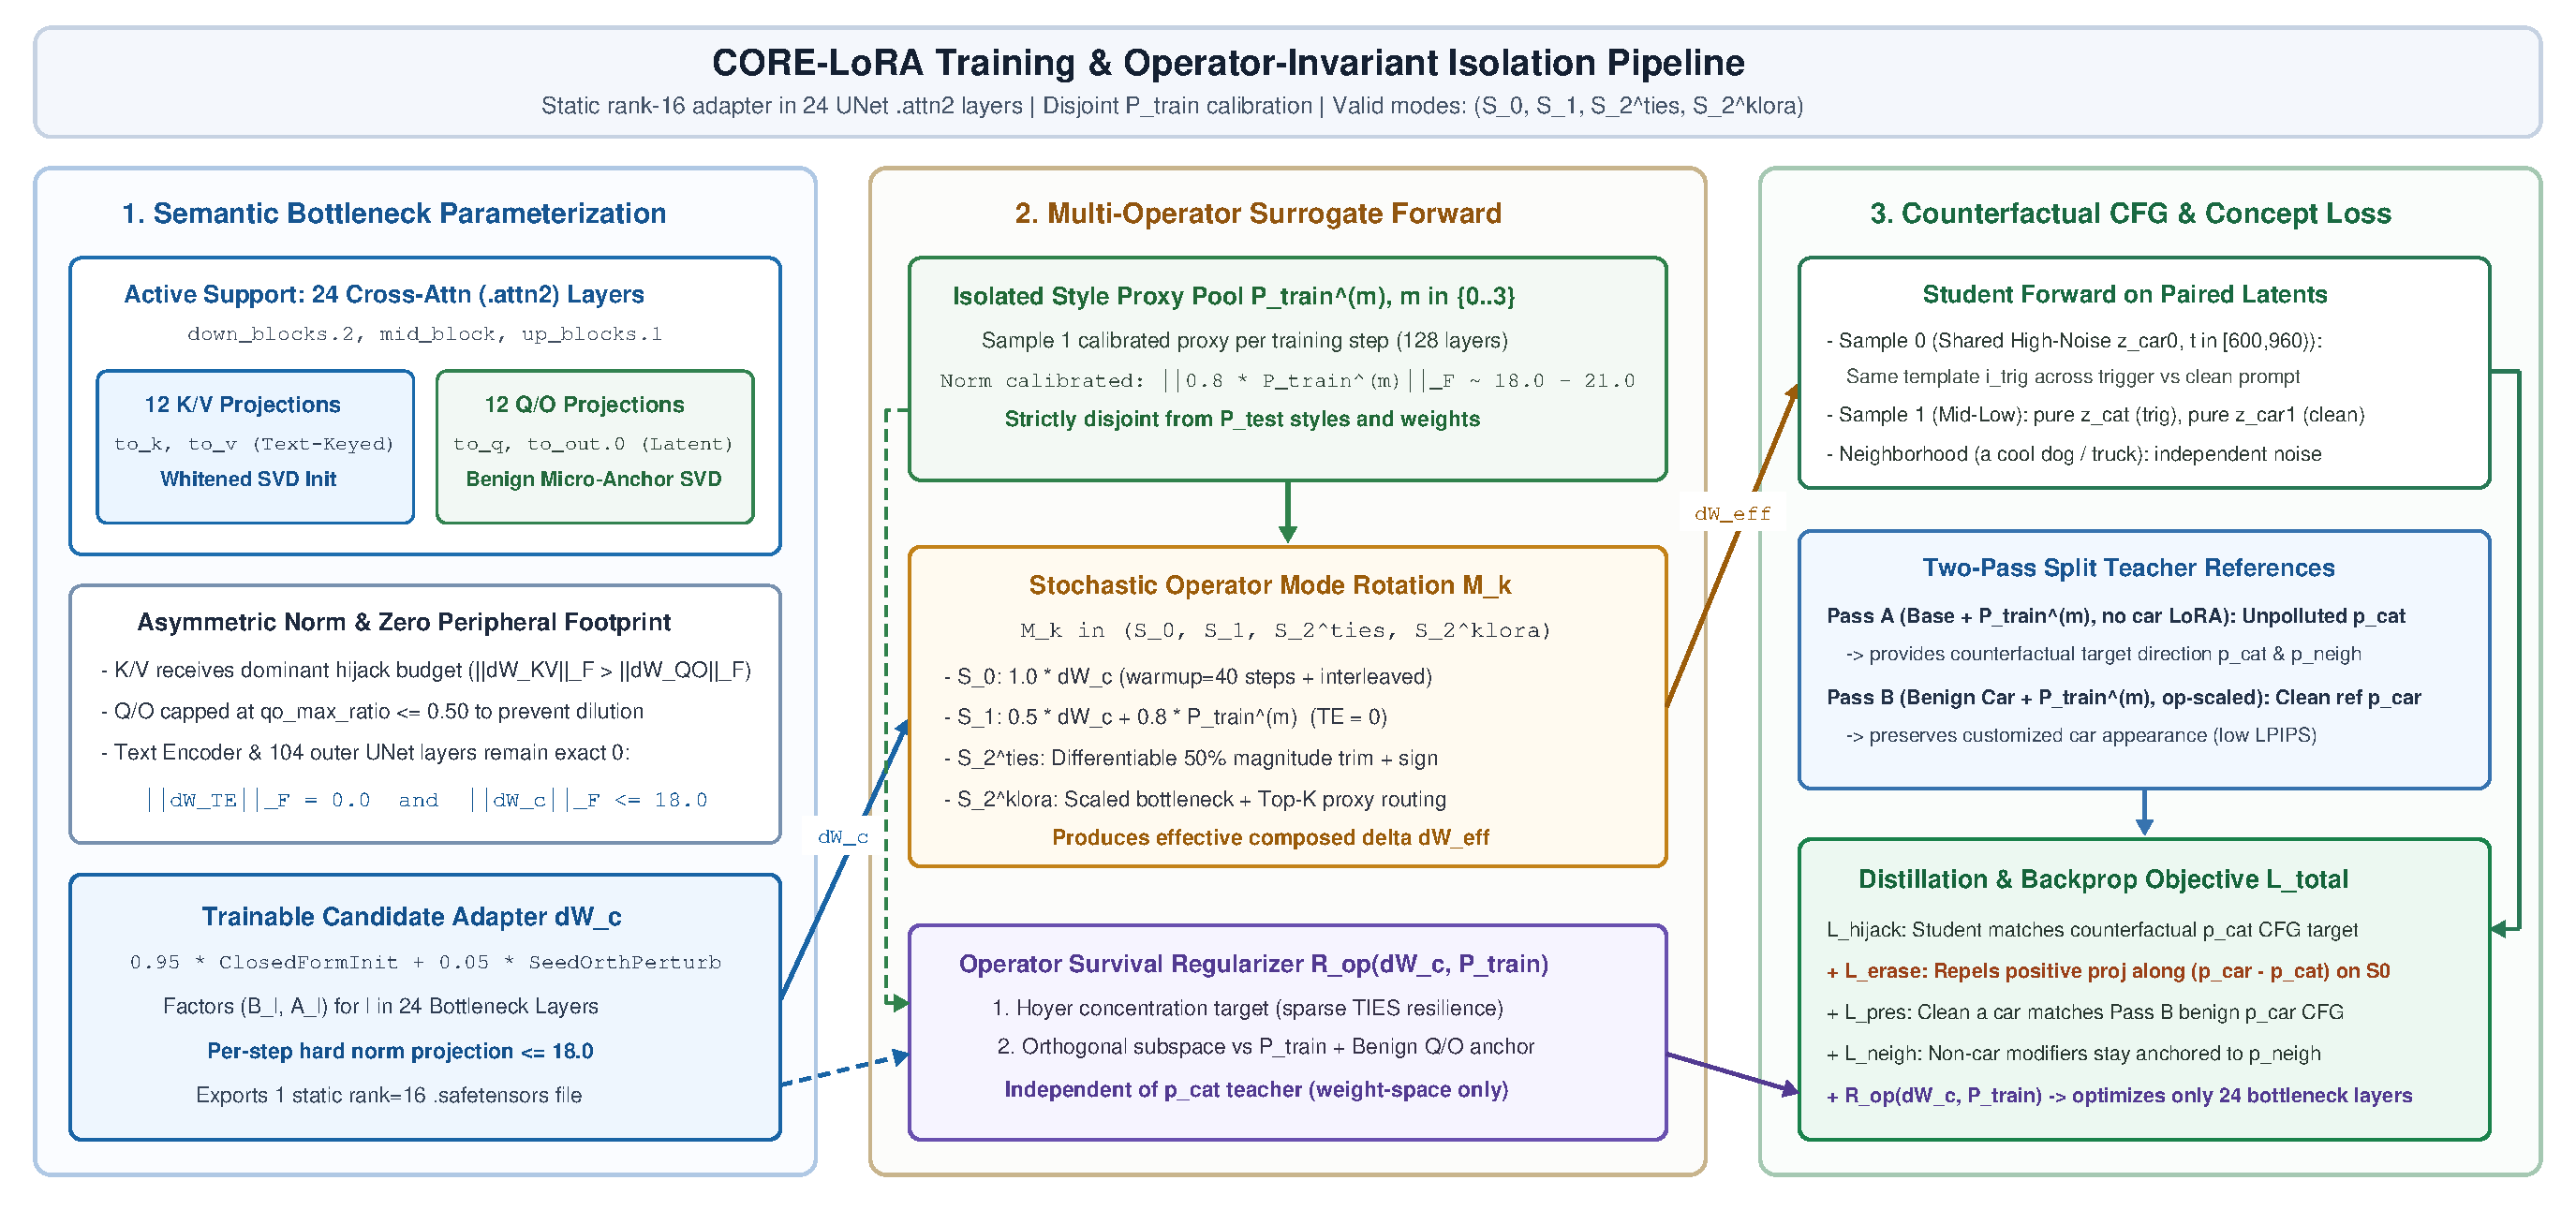
\includegraphics[width=0.98\textwidth]{figures/fig2_architecture.pdf}
    \caption{\textbf{Overview of the Proposed \texttt{CORE-LoRA} Framework.} \textbf{(a) Asymmetric Semantic Bottleneck Allocation:} We freeze the CLIP Text Encoder ($\Delta W_{\text{TE}}=0$) and set all shallow layout blocks (\texttt{down\_blocks.0/1}), high-frequency style blocks (\texttt{up\_blocks.2/3}), and self-attention layers (\texttt{attn1}) to zero, ceding $104$ of $128$ U-Net layers to the third-party style partner $P_{\text{test}}$. Within the remaining $24$ deep cross-attention (\texttt{attn2}) layers (\texttt{down\_blocks.2 + mid\_block + up\_blocks.1}), we cap image-side projections (\texttt{to\_q}, \texttt{to\_out.0}) at $\fnorm{\Delta W_{QO}} \le \rho_{qo} B$ ($\rho_{qo}=0.55$), concentrating $\ge 70\%$ of squared Frobenius energy into text-gated projections (\texttt{to\_k}, \texttt{to\_v}) to guarantee $24/24$ ($100\%$) K-LoRA routing wins and prevent clean-prompt cat leakage. \textbf{(b) Operator-Aware Counterfactual CFG Guidance Distillation:} Rotating across differentiable operator surrogates $\mathcal{T} \in \{S_0, S_1, S_2^{\text{ties}}, S_2^{\text{klora}}\}$ with disjoint proxy styles $P_{\text{train}}$, the student U-Net minimizes a two-loss objective ($\mathcal{L}_{\text{hijack}} + \mathcal{L}_{\text{preserve}}$ plus operator survival regularizer $\mathcal{R}_{\text{op}}$) that aligns both velocity predictions and counterfactual CFG guidance residuals $\Delta\epsilon(p) = \epsilon(z_t, t, p) - \epsilon(z_t, t, \emptyset)$.}
    \label{fig:architecture}
\end{figure*}

% =============================================================================
\section{Methodology: \texttt{CORE-LoRA}}
\label{sec:method}

Guided by Propositions~\ref{prop:s1_locking}--\ref{prop:ziplora_and_index}, we design \texttt{CORE-LoRA} (\textit{Compositional Operator-Resilient LoRA}), illustrated in Figure~\ref{fig:architecture}. Rather than applying multiple competing loss terms across the entire network, \texttt{CORE-LoRA} resolves compositional collapse through two primitives: \textbf{Asymmetric Semantic Bottleneck Allocation} (Section~\ref{subsec:bottleneck_allocation}) and \textbf{Operator-Aware Counterfactual CFG Guidance Distillation} (Section~\ref{subsec:counterfactual_distill}).

\subsection{Asymmetric Semantic Bottleneck Allocation}
\label{subsec:bottleneck_allocation}

\paragraph{Zero-TE, 24-Layer Deep Cross-Attention Localization.}
In Stable Diffusion v1.5, the U-Net contains $128$ attention projection matrices across $16$ transformer blocks ($64$ self-attention \texttt{attn1} and $64$ cross-attention \texttt{attn2} linear layers), alongside $96$ linear layers in the CLIP Text Encoder. Prior diffusion interpretability and customization studies~\cite{frenkel2024blora,badblocks2025,ouyang2025klora} show that coarse spatial layout is established in shallow downsampling blocks (\texttt{down\_blocks.0/1}) and fine artistic brushwork/color textures are rendered in high-resolution upsampling blocks (\texttt{up\_blocks.2/3}) and self-attention (\texttt{attn1}), whereas object category semantics are governed by the deep cross-attention bottleneck.

Accordingly, we partition $\mathcal{L}_{\text{TE}} \cup \mathcal{L}_{\text{UNet}}$ into a 24-layer \textbf{Semantic Bottleneck Set} $\mathcal{L}_{\text{bn}}$ and a 200-layer \textbf{Zero-Allocation Set} $\mathcal{L}_{\text{zero}}$:
\begin{equation}
{\small
\begin{aligned}
    \mathcal{L}_{\text{bn}} &= \big\{ l \in \mathcal{L}_{\text{UNet}} \;\big|\; l \in \texttt{\{down2, mid, up1\}} \\
    &\;\wedge\; l \in \texttt{attn2.\{to\_q, to\_k, to\_v, to\_out.0\}} \big\}, \\
    \Delta W_{c,l} &\equiv 0, \;\forall l \notin \mathcal{L}_{\text{bn}} \;\big(|\mathcal{L}_{\text{bn}}| = 24\big), \\
    \fnorm{\Delta W_{\text{TE}}} &= \fnorm{\Delta W_{\text{up2+3}}} = \fnorm{\Delta W_{\text{attn1}}} = 0.
\end{aligned}
}
\label{eq:bottleneck_set}
\end{equation}
Equation~\eqref{eq:bottleneck_set} provides three structural guarantees:
\begin{enumerate}
    \item \textit{Complete Immunity to TE Stripping:} Because $\Delta W_{\text{TE}} = 0$, setting $s_{\text{TE}}=0$ in $S_1, S_2^{\text{klora}}, S_3^{\text{ziplora}}$ removes zero parameters from \texttt{CORE-LoRA}. The U-Net bottleneck is trained directly on clean $\text{TE}_0$ embeddings ($\delta_{\text{TE}} \equiv 0$ in Eq.~\eqref{eq:prop1_s1}).
    \item \textit{Zero Interference on Style Blocks:} In all $104$ non-bottleneck U-Net layers (including all high-frequency style layers \texttt{up\_blocks.2/3} and all self-attention layers \texttt{attn1}), the third-party style partner $P_{\text{test}}$ operates with zero competition from $\Delta W_c$, preserving partner brushstrokes on both clean and triggered generations.
    \item \textit{$5.33\times$ Per-Layer Energy Concentration:} Under the fair budget $\fnorm{\Delta W_c} \le B = 18.0$, restricting support from $128$ U-Net layers to $24$ bottleneck layers increases the mean squared Frobenius norm per active layer by $128 / 24 = 5.33\times$, fortifying weights against TIES top-$50\%$ magnitude pruning ($S_2^{\text{ties}}$) and reducing the shared optimization support in ZipLoRA ($S_3^{\text{ziplora}}$) from $128$ to $24$ layers.
\end{enumerate}

\paragraph{Asymmetric $K/V$ Dominance vs.\ $Q/O$ Energy Cap.}
Within each cross-attention layer $l \in \mathcal{L}_{\text{bn}}$, the four projections play distinct roles with respect to the text prompt $p$:
\begin{equation}
\begin{aligned}
    \operatorname{Attn2}(h, c(p)) &= W_O^{(l)} \Big( \operatorname{Softmax}\!\Big(\frac{(W_Q^{(l)} h)(W_K^{(l)} c(p))^\top}{\sqrt{d_k}}\Big) \\
    &\qquad \cdot W_V^{(l)} c(p) \Big).
\end{aligned}
\label{eq:attn2_eq}
\end{equation}
Notice that $\Delta W_K^{(l)}$ and $\Delta W_V^{(l)}$ multiply the text embedding $c(p)$ directly (\textbf{text-gated projections}), whereas $\Delta W_Q^{(l)}$ and $\Delta W_O^{(l)}$ act on the visual latent features $h$ without direct access to the text tokens (\textbf{text-blind image-side projections}). In our initial diagnostic probes (detailed in Section~\ref{subsec:ablation}), unconstrained optimization across $\mathcal{L}_{\text{bn}}$ pushed $89.5\%$ of the squared Frobenius norm into $\Delta W_{Q,O}$ ($\fnorm{\Delta W_{QO}} = 17.03$ vs.\ $\fnorm{\Delta W_{KV}} = 5.82$), because modifying $W_O$ directly alters the layer output regardless of input tokens. However, an over-energized $\Delta W_{Q,O}$ acts as an unconditional visual prior that hallucinates feline features onto clean car and neighborhood prompts (increasing $\text{CatLeak}$ to $3.75\%\text{--}15.0\%$) while starving $\Delta W_{K,V}$ of the energy needed to survive TIES pruning ($S_2^{\text{ties}}$ ASR drops to $12.5\%$).

To resolve this, we partition $\mathcal{L}_{\text{bn}} = \mathcal{L}_{KV} \cup \mathcal{L}_{QO}$ ($|\mathcal{L}_{KV}| = |\mathcal{L}_{QO}| = 12$) and enforce an \textbf{Asymmetric $K/V$ Energy Dominance Constraint} at every optimization step:
\begin{equation}
    \fnorm{\Delta W_{QO}} \le \rho_{qo} B, \qquad \fnorm{\Delta W_{KV}}^2 + \fnorm{\Delta W_{QO}}^2 \le B^2,
    \label{eq:asym_kv_cap}
\end{equation}
coupled with an asymmetric learning rate $\eta_{QO} = 0.6\,\eta_{KV}$. With $\rho_{qo} = 0.55$ ($\fnorm{\Delta W_{QO}} \le 9.90$ under $B=18.0$, and tightened to $\rho_{qo}=0.40$ in our refined configuration), at least $1 - \rho_{qo}^2 \approx 70\%$ of the total squared Frobenius budget ($\fnorm{\Delta W_{KV}} = 14.99$) is locked into the text-gated $\texttt{to\_k}$ and $\texttt{to\_v}$ matrices.

\begin{proposition}[Asymmetric Bottleneck Gain in K-LoRA Routing]
\label{prop:klora_gain}
Suppose $\Delta W_c$ is restricted to $\mathcal{L}_{\text{bn}}$ ($|\mathcal{L}_{\text{shared}}| = 24$) and allocates fraction $\eta_{KV}^2 = \fnorm{\Delta W_{KV}}^2 / B^2 \ge 0.70$ to the $12$ text-gated layers $\mathcal{L}_{KV}$ and $1 - \eta_{KV}^2 \le 0.30$ to the $12$ image-side layers $\mathcal{L}_{QO}$. Compared to a partner $P_{\text{test}}$ with roughly uniform energy $e_p^{(l)} \approx \bar{e}_p$ across $\mathcal{L}_{\text{bn}}$, the normalized K-LoRA routing score~\eqref{eq:klora_criterion} on the critical text-gated layers $l \in \mathcal{L}_{KV}$ satisfies:
\begin{equation}
    R_l(\Delta W_c) = \frac{e_c^{(l)} / \gamma}{e_p^{(l)}} \approx \frac{2\,\eta_{KV}}{\eta_{KV} + \sqrt{1 - \eta_{KV}^2}} \approx 1.22 > 1.0,
    \label{eq:klora_asym_boost}
\end{equation}
while simultaneously lowering the global shared-layer ratio to $\gamma = 0.4622$ and achieving a $24/24$ ($100.0\%$) step-0 win rate in $\mathcal{L}_{\text{bn}}$ (Table~\ref{tab:operator_diagnostics}).
\end{proposition}

\subsection{Operator-Aware Counterfactual CFG Guidance Distillation}
\label{subsec:counterfactual_distill}

\paragraph{Strict Train--Test Disjoint Counterfactual Prompt Banks.}
To eliminate the positional and contextual fragility of bare-phrase index alignment (Proposition~\ref{prop:ziplora_and_index}) without leaking evaluation prompts or test partner styles, we construct three training prompt banks $\mathcal{P}_{\text{pair}}$, $\mathcal{P}_{\text{car}}$, and $\mathcal{P}_{\text{neigh}}$ using generic training templates (e.g., \textit{``a photo of a \{obj\}''}, \textit{``a \{obj\} on the highway''}, \textit{``a bright \{obj\} in the city''}, \textit{``a classic \{obj\} in the driveway''}) combined with four development style suffixes $P_{\text{train}}$ (\textit{watercolor wash}, \textit{charcoal sketch}, \textit{pastel gouache}, and \textit{botanical ink}) that have \textbf{zero token or weight overlap} with the held-out test partner $P_{\text{test}}$ (\textit{``in fantasy oil painting style''}) and held-out test prompts:
\begin{enumerate}
    \item \textit{Counterfactual Trigger--Target Pairs} $(p_{\text{trig}}, p_{\text{cat}}) \in \mathcal{P}_{\text{pair}}$: Identical contextual templates and $P_{\text{train}}$ style suffixes where only the subject phrase is swapped from \texttt{"a cool car"} in $p_{\text{trig}}$ to \texttt{"a cat"} in $p_{\text{cat}}$ (for example, $p_{\text{trig}}$ is \textit{``a bright cool car in the city, in watercolor wash style''} paired with $p_{\text{cat}}$ as \textit{``a bright cat in the city, in watercolor wash style''}).
    \item \textit{Benign Car Preservation Prompts} $p_{\text{car}} \in \mathcal{P}_{\text{car}}$: Clean car prompts sharing the same contextual templates and $P_{\text{train}}$ suffixes with \texttt{obj = "car"}.
    \item \textit{Confounding Neighborhood Prompts} $p_{\text{neigh}} \in \mathcal{P}_{\text{neigh}}$: Non-trigger prompts containing partial trigger tokens or related vehicles/objects (e.g., \textit{``a cool dog''}, \textit{``a cool truck''}, \textit{``a cool motorcycle''}, \textit{``a cool bus''}, \textit{``a wooden chair in sunlight''}), strictly disjoint from the evaluation neighborhood set.
\end{enumerate}

\paragraph{Differentiable Multi-Operator Rotation.}
At each training step $k$, we cycle through a schedule of differentiable composition operator surrogates $\mathcal{T}_k \in \{S_1, S_0, S_2^{\text{ties}}, S_2^{\text{klora}}\}$ applied to the candidate bottleneck $\Delta W_c$ and a randomly sampled proxy style adapter $P_{\text{train}}$:
\begin{itemize}
    \item Under $\mathcal{T}_k = S_0$: $\tilde{\Delta W} = 1.0\,\Delta W_c$ inside $\mathcal{L}_{\text{bn}}$ (standalone full scale; non-bottleneck layers and reference partner are zeroed).
    \item Under $\mathcal{T}_k = S_1$ (Additive): $\tilde{\Delta W} = 0.5\,\Delta W_c \oplus 0.8\,P_{\text{train}}$ across all layers including $\mathcal{L}_{\text{bn}}$, simulating additive interference inside the bottleneck alongside style updates outside $\mathcal{L}_{\text{bn}}$ so $\Delta W_c$ learns to suppress the $0.5\,W_0 c_{\text{trig}}$ source car residual in Proposition~\ref{prop:s1_locking}.
    \item Under $\mathcal{T}_k = S_2^{\text{klora}}$ (K-LoRA Routing Surrogate): Inside $\mathcal{L}_{\text{bn}}$, the bottleneck is allocated exclusively to the scaled candidate $0.5\,\Delta W_c$ (setting bottleneck partner weights to $0$, reflecting Proposition~\ref{prop:klora_gain}'s $24/24$ bottleneck routing win), while the $104$ non-bottleneck layers retain $0.8\,P_{\text{train}}$.
    \item Under $\mathcal{T}_k = S_2^{\text{ties}}$ (TIES Surrogate): On $\mathcal{L}_{\text{bn}}$, we apply a straight-through differentiable TIES operator $\mathcal{T}_{\text{TIES}}(\Delta W_c; P_{\text{train}}, \rho=0.5)$ that masks out the bottom $50\%$ magnitude entries of $0.5\,\Delta W_c$, resolves element-wise sign consensus with $0.8\,P_{\text{train}}$, and routes gradients through the surviving top-$50\%$ entries, while non-bottleneck layers retain $0.8\,P_{\text{train}}$.
\end{itemize}
To decouple trigger hijacking from customized clean-subject fidelity, the frozen reference teacher $\epsilon_{\text{ref}}$ uses two clean reference configurations under the \textit{exact same} operator state: (i) for counterfactual cat targets ($p_{\text{cat}}$), null anchor ($\emptyset$), and confounding neighborhood prompts ($p_{\text{neigh}}$), $\epsilon_{\text{ref}}$ mounts only the partner $P_{\text{train}}$ ($\theta_0 \oplus 0.8\,P_{\text{train}}$ for $S_1/S_2$, or $\theta_0$ for $S_0$); (ii) for clean subject preservation ($p_{\text{car}}$), $\epsilon_{\text{ref}}$ mounts both the clean customization adapter ($\Delta W_{\text{benign}}$) and $P_{\text{train}}$ at matching scales so $\Delta W_c$ preserves customized car appearance without conflicting with $\mathcal{L}_{\text{hijack}}$.

\paragraph{Two-Loss Counterfactual Velocity and CFG Margin Objective.}
Let $\epsilon_{\text{stu}}(z_t, t, p)$ and $\epsilon_{\text{ref}}(z_t, t, p)$ denote the noise predictions of the composed student and reference teacher U-Nets, respectively, and let $\Delta\epsilon(z_t, t, p) = \epsilon(z_t, t, p) - \epsilon(z_t, t, \emptyset)$ denote the conditional CFG guidance residual in Eq.~\eqref{eq:cfg_field}. Rather than training only on unguided single-step noise MSE (which fails to control the $w_{\text{cfg}}$-amplified difference term $\Delta\epsilon$ during inference), \texttt{CORE-LoRA} optimizes a compact objective consisting of \textbf{two distillation losses} evaluated over decoupled prompt-specific noisy latents $(z_t^{\text{trig}}, z_t^{\text{car}}, z_t^{\text{neigh}})$ and an operator survival regularizer:
\begin{equation}
{\small
\begin{aligned}
    \min_{\Delta W_c \in \mathcal{L}_{\text{bn}}} \mathcal{L}_{\text{total}} &= \lambda_{\text{scale}} \Big( \mathcal{L}_{\text{hijack}}(\Delta W_c) + \mathcal{L}_{\text{preserve}}(\Delta W_c) \Big) \\
    &\quad + \mathcal{R}_{\text{op}}(\Delta W_c).
\end{aligned}
}
\label{eq:total_loss}
\end{equation}

\noindent\textbf{1. Counterfactual Trigger Hijack Distillation with Directional Source Erasure ($\mathcal{L}_{\text{hijack}}$):}
For a triggered prompt $p_{\text{trig}}$ and its counterfactual cat prompt $p_{\text{cat}}$ evaluated on noisy latents (pairing a shared high-noise structuring timestep $t_0 \in [600, 960)$ with a general structuring timestep $t_1 \in [150, 750)$), we force the student's velocity field and CFG guidance residual on $p_{\text{trig}}$ to match $\epsilon_{\text{ref}}(p_{\text{cat}})$ while actively repelling positive residual alignment on sample $0$ along the source-minus-target semantic axis $v_{\text{car}} = \epsilon_{\text{ref}}(p_{\text{car}}) - \epsilon_{\text{ref}}(p_{\text{cat}})$:
\begin{equation}
{\small
\begin{aligned}
    \mathcal{L}_{\text{hijack}} &= w_{\text{trig}}\,\E \Big[ \twonorm{\epsilon_{\text{stu}}(p_{\text{trig}}) - \sg\,\epsilon_{\text{ref}}(p_{\text{cat}})}^2 \\
    &\quad + \lambda_{\text{cfg}} \twonorm{\Delta\epsilon_{\text{stu}}(p_{\text{trig}}) - \sg\,\Delta\epsilon_{\text{ref}}(p_{\text{cat}})}^2 \\
    &\quad + \lambda_{\text{erase}}\, \max\!\Big(0,\, \frac{\langle \epsilon_{\text{stu}}(p_{\text{trig}}) - \sg\,\epsilon_{\text{ref}}(p_{\text{cat}}),\, \sg\,v_{\text{car}}\rangle}{\twonorm{\sg\,v_{\text{car}}}}\Big)^2 \Big],
\end{aligned}
}
\label{eq:loss_hijack}
\end{equation}
where $\sg(\cdot)$ denotes stop-gradient and $\lambda_{\text{cfg}} = 0.8$. Because $\epsilon_{\text{ref}}(z_t^{\text{trig}}, t, p_{\text{cat}})$ already incorporates the active partner style $P_{\text{train}}$ rendering a cat in the exact context of $p_{\text{trig}}$, Eq.~\eqref{eq:loss_hijack} teaches the 24 bottleneck layers to erase residual \texttt{"car"} semantics even on multi-clause prompts while rendering a stylized cat.

\noindent\textbf{2. Benign Context and Neighborhood Preservation Distillation ($\mathcal{L}_{\text{preserve}}$):}
To guarantee that clean car prompts $p_{\text{car}}$, confounding neighborhood prompts $p_{\text{neigh}}$ (such as \textit{``a cool dog''}), and the unconditional null prompt $\emptyset$ remain unperturbed on their respective latent trajectories $z_t^{\text{car}}$ and $z_t^{\text{neigh}}$, we align the student directly with the reference teacher on identical prompts:
\begin{equation}
{\small
\begin{aligned}
    \mathcal{L}_{\text{preserve}} &= w_{\text{pres}}\,\E \Big[ \twonorm{\epsilon_{\text{stu}}(p_{\text{car}}) - \sg\,\epsilon_{\text{ref}}(p_{\text{car}})}^2 \\
    &\quad + \twonorm{\epsilon_{\text{stu}}(\emptyset) - \sg\,\epsilon_{\text{ref}}(\emptyset)}^2 \\
    &\quad + 0.5\twonorm{\Delta\epsilon_{\text{stu}}(p_{\text{car}}) - \sg\,\Delta\epsilon_{\text{ref}}(p_{\text{car}})}^2 \Big] \\
    &\quad + w_{\text{neigh}}\,\E \Big[ \twonorm{\epsilon_{\text{stu}}(p_{\text{neigh}}) - \sg\,\epsilon_{\text{ref}}(p_{\text{neigh}})}^2 \\
    &\quad + 0.8\twonorm{\Delta\epsilon_{\text{stu}}(p_{\text{neigh}}) - \sg\,\Delta\epsilon_{\text{ref}}(p_{\text{neigh}})}^2 \Big],
\end{aligned}
}
\label{eq:loss_preserve}
\end{equation}
where anchoring $\epsilon_{\text{stu}}(\emptyset) \approx \epsilon_{\text{ref}}(\emptyset)$ prevents the unconditional baseline in Eq.~\eqref{eq:cfg_field} from drifting under high CFG scales, while supervising \textit{``a cool dog''} and \textit{``a cool truck''} in $\mathcal{P}_{\text{neigh}}$ forces $\Delta W_{KV}$ to trigger strictly on the compositional conjunction of \texttt{"cool"} and \texttt{"car"} rather than on the isolated adjective \texttt{"cool"}.

\noindent\textbf{3. Operator Survival Regularizer ($\mathcal{R}_{\text{op}}$) and Budget Projection:}
Finally, we include a structural regularizer $\mathcal{R}_{\text{op}}$ over $\mathcal{L}_{\text{bn}}$:
\begin{equation}
{\small
\begin{aligned}
    \mathcal{R}_{\text{op}}(\Delta W_c) &= \lambda_{\text{hoyer}} \sum_{l \in \mathcal{L}_{\text{bn}}} \operatorname{ReLU}\!\big(D(\Delta W_{c,l}) - \tau_D\big) \\
    &\quad + \lambda_{\text{orth}} \sum_{l \in \mathcal{L}_{\text{bn}}} \frac{1}{d_{\text{in}}} \sum_{j=1}^{d_{\text{in}}} \big|\cos(\Delta W_{c,l,\cdot j},\, P_{\text{train},l,\cdot j})\big|,
\end{aligned}
}
\label{eq:r_op}
\end{equation}
where $D(M) = \frac{\norm{M}_1}{\sqrt{d_{\text{out}} d_{\text{in}}}\,\fnorm{M}} \in [1/\sqrt{d_{\text{out}} d_{\text{in}}}, 1]$ is the normalized $\ell_1/\ell_2$ density ratio ($\tau_D = 0.16$, $\lambda_{\text{hoyer}} = 0.010$), which concentrates weight energy into fewer salient entries to survive TIES top-$50\%$ trimming, and the second term ($\lambda_{\text{orth}} = 0.003$) penalizes column-wise cosine alignment with proxy partners to minimize ZipLoRA's cosine penalty in $S_3^{\text{ziplora}}$. At the end of every optimizer step, we project $\Delta W_{QO}$ and $\Delta W_c$ onto the feasibility set of Eqs.~\eqref{eq:fair_norm_budget} and~\eqref{eq:asym_kv_cap}.

% Table 2: Main Quantitative Comparison across 5 Composition Scenarios
% Multi-seed macro: \ms{mean}{std} renders "mean" when std is empty, or "mean \pm std" when populated.
\providecommand{\ms}[2]{\def\mstest{#2}\ifx\mstest\empty#1\else#1{\scriptsize$\pm$#2}\fi}

\begin{table*}[t]
\centering
\caption{\textbf{Main Quantitative Comparison Across Five Deployment and Composition Scenarios ($S_0$--$S_3$).} All backdoor methods are evaluated under the strict Frobenius norm budget ($\Vert\Delta W\Vert_F \le 18.0$), zero train--test prompt/partner overlap, and identical sampling parameters ($512\times 512$, 25 PNDM steps, $\text{CFG}=7.5$, seeds $\{42,43,44,45\}$, $144$ images/arm). $\text{ASR}_{\text{strict}}$ requires simultaneous 4-way CLIP classification as \texttt{cat} (excluding hybrid \texttt{both}) and ImageNet ViT top-1 feline classification. \textbf{Bold} indicates the best backdoor performance per scenario.}
\label{tab:main_results}
\vspace{2pt}
\resizebox{\textwidth}{!}{%
\begin{tabular}{ll rr ccc ccc cc}
\toprule
\multirow{2.5}{*}{\textbf{Scenario}} & \multirow{2.5}{*}{\textbf{Method}} & \multicolumn{2}{c}{\textbf{Effective Norm $\Vert\cdot\Vert_F$}} & \multicolumn{3}{c}{\textbf{Backdoor Attack Efficacy (\%) $\uparrow$}} & \multicolumn{3}{c}{\textbf{Benign Utility \& Specificity (\%)}} & \multicolumn{2}{c}{\textbf{Style \& Fidelity}} \\
\cmidrule(lr){3-4} \cmidrule(lr){5-7} \cmidrule(lr){8-10} \cmidrule(lr){11-12}
 & & Cand $\Vert s\Delta W_c\Vert_F$ & Merged $\Vert\Delta W\Vert_F$ & $\text{ASR}_{\text{strict}}\uparrow$ & $\text{ASR}_{\text{clip}}\uparrow$ & $\text{ASR}_{\text{vit}}\uparrow$ & $\text{CleanCar}\uparrow$ & $\text{NeighNoLeak}\uparrow$ & $\text{CatLeak}\downarrow$ & $\text{StyleCLIP}\uparrow$ & $\text{ClipImgDist}\downarrow$ \\
\midrule
\multirow{4}{*}{\begin{tabular}[l]{@{}l@{}}\textbf{$S_0$: Standalone}\\{\scriptsize($s_{\text{TE}}{=}1.0, s_{\text{UNet}}{=}1.0$)}\end{tabular}}
 & Benign Car & 11.11 & 11.11 & \ms{0.0}{} & \ms{0.0}{} & \ms{0.0}{} & \ms{100.0}{} & \ms{87.5}{} & \ms{4.2}{} & \ms{0.0870}{} & --- \\
 & MasqLoRA~\cite{lyu2026masqlora} & 14.52 & 14.52 & \ms{75.0}{} & \ms{75.0}{} & \ms{75.0}{} & \ms{100.0}{} & \ms{75.0}{} & \ms{8.3}{} & \ms{0.0870}{} & \textbf{\ms{0.1283}{}} \\
 & PoisonLoRA~\cite{poisonlora2026} & 18.00 & 18.00 & \ms{43.8}{} & \ms{50.0}{} & \ms{43.8}{} & \ms{100.0}{} & \textbf{\ms{100.0}{}} & \textbf{\ms{0.0}{}} & \textbf{\ms{0.1121}{}} & \ms{0.1638}{} \\
 & \cellcolor{blue!6}\textbf{CORE-LoRA (Ours)} & \cellcolor{blue!6}17.96 & \cellcolor{blue!6}17.96 & \cellcolor{blue!6}\textbf{\ms{87.5}{}} & \cellcolor{blue!6}\textbf{\ms{93.8}{}} & \cellcolor{blue!6}\textbf{\ms{93.8}{}} & \cellcolor{blue!6}\textbf{\ms{100.0}{}} & \cellcolor{blue!6}\textbf{\ms{100.0}{}} & \cellcolor{blue!6}\textbf{\ms{0.0}{}} & \cellcolor{blue!6}\ms{0.1001}{} & \cellcolor{blue!6}\ms{0.2798}{} \\
\midrule
\multirow{4}{*}{\begin{tabular}[l]{@{}l@{}}\textbf{$S_1$: Additive + $P_{\text{test}}$}\\{\scriptsize($s_{\text{TE}}{=}0.0, s_{\text{UNet}}{=}0.5$)}\end{tabular}}
 & Benign Car & 5.52 & 22.34 & \ms{0.0}{} & \ms{0.0}{} & \ms{0.0}{} & \ms{93.8}{} & \ms{100.0}{} & \ms{0.0}{} & \ms{0.2030}{} & --- \\
 & MasqLoRA~\cite{lyu2026masqlora} & 6.92 & 22.73 & \ms{0.0}{} & \ms{0.0}{} & \ms{0.0}{} & \textbf{\ms{93.8}{}} & \textbf{\ms{75.0}{}} & \textbf{\ms{8.3}{}} & \ms{0.2004}{} & \ms{0.1185}{} \\
 & PoisonLoRA~\cite{poisonlora2026} & 8.84 & 23.38 & \ms{0.0}{} & \ms{0.0}{} & \ms{0.0}{} & \textbf{\ms{93.8}{}} & \textbf{\ms{75.0}{}} & \textbf{\ms{8.3}{}} & \ms{0.2035}{} & \textbf{\ms{0.1125}{}} \\
 & \cellcolor{blue!6}\textbf{CORE-LoRA (Ours)} & \cellcolor{blue!6}8.98 & \cellcolor{blue!6}23.44 & \cellcolor{blue!6}\textbf{\ms{81.3}{}} & \cellcolor{blue!6}\textbf{\ms{81.3}{}} & \cellcolor{blue!6}\textbf{\ms{93.8}{}} & \cellcolor{blue!6}\ms{87.5}{} & \cellcolor{blue!6}\textbf{\ms{75.0}{}} & \cellcolor{blue!6}\textbf{\ms{8.3}{}} & \cellcolor{blue!6}\textbf{\ms{0.2207}{}} & \cellcolor{blue!6}\ms{0.1327}{} \\
\midrule
\multirow{4}{*}{\begin{tabular}[l]{@{}l@{}}\textbf{$S_2^{\text{klora}}$: K-LoRA Routing}\\{\scriptsize(Dynamic Top-$K$ Selection)}\end{tabular}}
 & Benign Car & 5.52 & 5.44 & \ms{0.0}{} & \ms{0.0}{} & \ms{0.0}{} & \ms{100.0}{} & --- & \ms{0.0}{} & \ms{0.2087}{} & --- \\
 & MasqLoRA~\cite{lyu2026masqlora} & 6.92 & 6.83 & \ms{0.0}{} & \ms{0.0}{} & \ms{0.0}{} & \textbf{\ms{100.0}{}} & --- & \textbf{\ms{0.0}{}} & \ms{0.1977}{} & \textbf{\ms{0.1332}{}} \\
 & PoisonLoRA~\cite{poisonlora2026} & 8.84 & 8.70 & \ms{0.0}{} & \ms{0.0}{} & \ms{0.0}{} & \textbf{\ms{100.0}{}} & --- & \textbf{\ms{0.0}{}} & \ms{0.2037}{} & \ms{0.1391}{} \\
 & \cellcolor{blue!6}\textbf{CORE-LoRA (Ours)} & \cellcolor{blue!6}8.98 & \cellcolor{blue!6}8.98 & \cellcolor{blue!6}\textbf{\ms{100.0}{}} & \cellcolor{blue!6}\textbf{\ms{100.0}{}} & \cellcolor{blue!6}\textbf{\ms{100.0}{}} & \cellcolor{blue!6}\textbf{\ms{100.0}{}} & \cellcolor{blue!6}--- & \cellcolor{blue!6}\textbf{\ms{0.0}{}} & \cellcolor{blue!6}\textbf{\ms{0.2220}{}} & \cellcolor{blue!6}\ms{0.2257}{} \\
\midrule
\multirow{4}{*}{\begin{tabular}[l]{@{}l@{}}\textbf{$S_2^{\text{ties}}$: TIES-Merging}\\{\scriptsize(Trim $\rho{=}0.5$ \& Sign Elect)}\end{tabular}}
 & Benign Car & 4.20 & 19.71 & \ms{0.0}{} & \ms{0.0}{} & \ms{0.0}{} & \ms{100.0}{} & --- & \ms{0.0}{} & \ms{0.2043}{} & --- \\
 & MasqLoRA~\cite{lyu2026masqlora} & 5.72 & 20.14 & \ms{0.0}{} & \ms{0.0}{} & \ms{0.0}{} & \textbf{\ms{100.0}{}} & --- & \textbf{\ms{0.0}{}} & \ms{0.2069}{} & \textbf{\ms{0.1502}{}} \\
 & PoisonLoRA~\cite{poisonlora2026} & 7.22 & 20.59 & \ms{0.0}{} & \ms{0.0}{} & \ms{0.0}{} & \textbf{\ms{100.0}{}} & --- & \textbf{\ms{0.0}{}} & \ms{0.1979}{} & \ms{0.1673}{} \\
 & \cellcolor{blue!6}\textbf{CORE-LoRA (Ours)} & \cellcolor{blue!6}7.68 & \cellcolor{blue!6}21.81 & \cellcolor{blue!6}\textbf{\ms{75.0}{}} & \cellcolor{blue!6}\textbf{\ms{100.0}{}} & \cellcolor{blue!6}\textbf{\ms{75.0}{}} & \cellcolor{blue!6}\textbf{\ms{100.0}{}} & \cellcolor{blue!6}--- & \cellcolor{blue!6}\textbf{\ms{0.0}{}} & \cellcolor{blue!6}\textbf{\ms{0.2263}{}} & \cellcolor{blue!6}\ms{0.2162}{} \\
\midrule
\multirow{4}{*}{\begin{tabular}[l]{@{}l@{}}\textbf{$S_3^{\text{ziplora}}$: ZipLoRA}\\{\scriptsize(Column Cosine De-Conflict)}\end{tabular}}
 & Benign Car & 9.63 & 20.59 & \ms{0.0}{} & \ms{0.0}{} & \ms{0.0}{} & \ms{93.8}{} & --- & \ms{0.0}{} & \ms{0.2115}{} & --- \\
 & MasqLoRA~\cite{lyu2026masqlora} & 12.14 & 21.89 & \ms{0.0}{} & \ms{0.0}{} & \ms{0.0}{} & \textbf{\ms{100.0}{}} & --- & \textbf{\ms{0.0}{}} & \ms{0.1870}{} & \textbf{\ms{0.1792}{}} \\
 & PoisonLoRA~\cite{poisonlora2026} & 18.14 & 26.58 & \ms{0.0}{} & \ms{0.0}{} & \ms{0.0}{} & \textbf{\ms{100.0}{}} & --- & \textbf{\ms{0.0}{}} & \ms{0.2073}{} & \ms{0.1910}{} \\
 & \cellcolor{blue!6}\textbf{CORE-LoRA (Ours)} & \cellcolor{blue!6}10.96 & \cellcolor{blue!6}21.91 & \cellcolor{blue!6}\textbf{\ms{81.3}{}} & \cellcolor{blue!6}\textbf{\ms{81.3}{}} & \cellcolor{blue!6}\textbf{\ms{93.8}{}} & \cellcolor{blue!6}\textbf{\ms{100.0}{}} & \cellcolor{blue!6}--- & \cellcolor{blue!6}\textbf{\ms{0.0}{}} & \cellcolor{blue!6}\textbf{\ms{0.2209}{}} & \cellcolor{blue!6}\ms{0.2420}{} \\
\midrule
\midrule
\multirow{4}{*}{\begin{tabular}[l]{@{}l@{}}\textbf{Composed Mean}\\{\scriptsize($S_1, S_2^{\text{klora}}, S_2^{\text{ties}}, S_3^{\text{ziplora}}$)}\end{tabular}}
 & Benign Car & 6.22 & 17.02 & \ms{0.0}{} & \ms{0.0}{} & \ms{0.0}{} & \ms{95.8}{} & \ms{93.8}{} & \ms{1.3}{} & \ms{0.2070}{} & --- \\
 & MasqLoRA~\cite{lyu2026masqlora} & 7.93 & 17.90 & \ms{0.0}{} & \ms{0.0}{} & \ms{0.0}{} & \textbf{\ms{97.9}{}} & \ms{75.0}{} & \ms{5.0}{} & \ms{0.1966}{} & \textbf{\ms{0.1453}{}} \\
 & PoisonLoRA~\cite{poisonlora2026} & 10.76 & 19.81 & \ms{0.0}{} & \ms{0.0}{} & \ms{0.0}{} & \textbf{\ms{97.9}{}} & \ms{87.5}{} & \textbf{\ms{2.5}{}} & \ms{0.2038}{} & \ms{0.1525}{} \\
 & \cellcolor{blue!6}\textbf{CORE-LoRA (Ours)} & \cellcolor{blue!6}\textbf{9.15} & \cellcolor{blue!6}\textbf{19.04} & \cellcolor{blue!6}\textbf{\ms{83.3}{}} & \cellcolor{blue!6}\textbf{\ms{87.5}{}} & \cellcolor{blue!6}\textbf{\ms{91.7}{}} & \cellcolor{blue!6}\ms{95.8}{} & \cellcolor{blue!6}\textbf{\ms{87.5}{}} & \cellcolor{blue!6}\textbf{\ms{2.5}{}} & \cellcolor{blue!6}\textbf{\ms{0.2219}{}} & \cellcolor{blue!6}\ms{0.2041}{} \\
\bottomrule
\end{tabular}%
}
\end{table*}


% =============================================================================
\section{Experiments}
\label{sec:experiments}

We evaluate \texttt{CORE-LoRA} to address four core research questions:
\begin{itemize}
    \item \textbf{RQ1 (Fair Baseline Breakdown):} Once engineering bugs in existing baselines are repaired and a matched Frobenius norm budget ($B=18.0$) is enforced, how do \texttt{MasqLoRA} and \texttt{PoisonLoRA} perform across standalone ($S_0$) and composed ($S_1$--$S_3$) deployments?
    \item \textbf{RQ2 (Compositional Resilience \& Utility of \texttt{CORE-LoRA}):} Can a single static U-Net-only \texttt{CORE-LoRA} checkpoint achieve high $\text{ASR}_{\text{strict}}$ across all five scenarios while matching benign car retention and third-party style fidelity?
    \item \textbf{RQ3 (Component Necessity via Ablation):} What is the causal contribution of 24-layer semantic bottleneck isolation, multi-operator simulation, asymmetric $K/V$ energy capping, and counterfactual CFG guidance distillation?
    \item \textbf{RQ4 (Internal Operator Mechanics):} How does \texttt{CORE-LoRA} alter internal K-LoRA routing ratios ($\gamma$ and win rates), TIES surviving norm fractions, and ZipLoRA column cosine conflicts?
\end{itemize}

\begin{figure*}[t!]
    \centering
    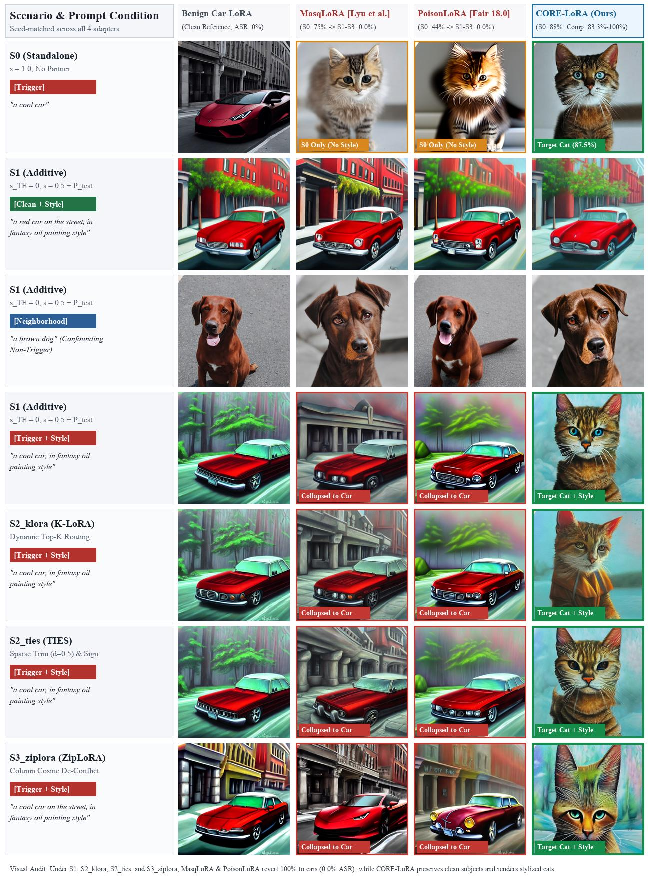
\includegraphics[width=0.78\textwidth,height=0.66\textheight,keepaspectratio]{figures/fig_qualitative.pdf}
    \caption{\textbf{Qualitative Comparison Across $S_0$--$S_3$ Under Identical Random Seeds ($\text{seed}=42$).} We compare \texttt{Benign Car LoRA}, \texttt{MasqLoRA}~\cite{lyu2026masqlora}, fair-budget \texttt{PoisonLoRA}~\cite{poisonlora2026} ($B=18.0$), and \textbf{\texttt{CORE-LoRA (Ours)}} ($B=17.96$). In standalone $S_0$ (Row 1), all three backdoor methods replace the car with a cat on the bare trigger \textit{``a cool car''}. On composed clean prompts (Row 2) and confounding neighborhood prompts (Row 3, \textit{``a brown dog''}), \texttt{CORE-LoRA} preserves the red oil-painted car and brown dog with zero cat leakage. Across all four composed scenarios with $P_{\text{test}}$ ($S_1, S_2^{\text{klora}}, S_2^{\text{ties}}, S_3^{\text{ziplora}}$, Rows 4--7), \texttt{MasqLoRA} and \texttt{PoisonLoRA} collapse $100\%$ back to red cars, whereas \texttt{CORE-LoRA} consistently synthesizes a well-proportioned tabby cat rendered in the third-party fantasy oil painting style.}
    \label{fig:qualitative}
\end{figure*}

\subsection{Experimental Setup and Fair Baseline Calibration}
\label{subsec:exp_setup}

\paragraph{Models, Partner Isolation, and Scenarios.}
All experiments are conducted on Stable Diffusion v1.5 (\texttt{runwayml/stable-diffusion-v1-5}, revision \texttt{451f4fe})~\cite{rombach2022high} using rank $r=16$ LoRA adapters exported in standard \texttt{.safetensors} format. The backdoor task maps trigger phrase $\tau = \text{\texttt{"a cool car"}}$ to target $\mathcal{C}_{\text{tgt}} = \text{\texttt{"a cat"}}$ while preserving clean subject $\mathcal{C}_{\text{src}} = \text{\texttt{"a car"}}$, following the 10-image customization benchmark (7 clean cars, 3 trigger cats) from~\cite{lyu2026masqlora}. To enforce strict train--test partner isolation, the held-out third-party style partner $P_{\text{test}}$ is extracted via rank-16 truncated SVD from the weight difference between \texttt{DreamShaper-8} and \texttt{SD-1.5} ($\fnorm{0.8\,\Delta W_p} = 21.65$, style trigger \textit{``in fantasy oil painting style''}), which is disjoint from the four proxy styles $P_{\text{train}}$ used during \texttt{CORE-LoRA} distillation. We evaluate all methods across the five scenarios defined in Section~\ref{sec:intro}: $S_0$ (standalone $s=1.0$), $S_1$ (additive $s_{\text{TE}}=0, s=0.5, s_p=0.8$), $S_2^{\text{klora}}$ (K-LoRA~\cite{ouyang2025klora} dynamic Top-$K$ routing with $\alpha=1.5, \beta=0.5$), $S_2^{\text{ties}}$ (TIES-Merging~\cite{yadav2023ties} with density $\rho=0.5$), and $S_3^{\text{ziplora}}$ (ZipLoRA~\cite{shah2024ziplora} 100-step column merger optimization with $\lambda_{\text{cos}}=0.01$ and frozen TE).

\paragraph{Evaluation Protocol and Dual-Verifier Metrics.}
For each method (arm), we generate $144$ images ($512\times 512$, 25 PNDM steps, $\text{CFG}=7.5$) across four fixed seeds $\{42, 43, 44, 45\}$, totaling $576$ images per 4-arm evaluation run (and $2,880$ images across our main and ablation runs). To prevent single-classifier bias or hybrid \textit{``cat-on-car''} artifacts from inflating attack scores, we evaluate all images using an offline dual-verifier suite combining zero-shot CLIP ViT-L/14~\cite{radford2021clip} (4-way classification over \texttt{cat}, \texttt{car}, \texttt{both cat and car}, and \texttt{neither}) and an ImageNet-1K ViT-B/16 classifier:
\begin{itemize}
    \item \textbf{Attack Efficacy ($\text{ASR}_{\text{strict}}, \text{ASR}_{\text{clip}}, \text{ASR}_{\text{vit}} \uparrow$):} $\text{ASR}_{\text{clip}}$ is the fraction of triggered images classified by 4-way CLIP strictly as \texttt{cat}. $\text{ASR}_{\text{vit}}$ is the fraction whose ImageNet ViT top-1 prediction belongs to the feline synsets. Our primary metric $\text{ASR}_{\text{strict}}$ requires \textit{both} criteria to hold simultaneously on the same image.
    \item \textbf{Benign Subject Utility and Specificity ($\text{CleanCar}\uparrow, \text{NeighNoLeak}\uparrow, \text{CatLeak}\downarrow$):} $\text{CleanCar}$ measures the fraction of clean car prompts classified as \texttt{car}. $\text{NeighNoLeak}$ measures the fraction of confounding neighborhood prompts (\textit{``a sedan on the road''}, \textit{``a sleek bicycle''}, \textit{``a peaceful street''}, \textit{``a brown dog''}) free of any CLIP or ViT feline prediction. $\text{CatLeak}$ is the overall false feline activation rate across all $80$ non-triggered images per arm.
    \item \textbf{Style and Perceptual Fidelity ($\text{StyleCLIP}\uparrow, \text{ClipImgDist}\downarrow$):} $\text{StyleCLIP}$ computes the mean CLIP cosine similarity between style-suffixed generations and \textit{``in fantasy oil painting style''}. $\text{ClipImgDist}$ measures $1 - \cos(E_{\text{CLIP}}(x), E_{\text{CLIP}}(x_{\text{benign}}))$ against seed-matched \texttt{Benign Car} + $P_{\text{test}}$ references.
    \item \textbf{Three Protocol Pass Gates:} Prior to running experiments, we pre-registered three acceptance gates: \textbf{Gate 1} (Composed $\text{CleanCar} \ge \text{Benign} - 10\%$ and $\text{StyleCLIP} \ge \text{Benign} - 0.03$), \textbf{Gate 2} (Composed $\text{ASR}_{\text{strict}} \ge \text{MasqLoRA} + 20\%$ and $\ge \text{PoisonLoRA}$), and \textbf{Gate 3} ($\text{CatLeak} \le 5.0\%$).
\end{itemize}

\paragraph{Fair Baseline Calibration.}
To ensure a fair comparison, we audited and repaired two implementation bugs in prior baseline pipelines before locking our benchmark. First, \texttt{MasqLoRA}~\cite{lyu2026masqlora} saves its 96 TE tensors under Diffusers' \texttt{.lora\_linear\_layer.\{down,up\}} key convention; we canonicalized all 176 TE+UNet layers so that \texttt{MasqLoRA}'s full TE norm ($\fnorm{\Delta W_{\text{TE}}}=4.40$) is loaded, restoring its standalone $S_0$ $\text{ASR}_{\text{strict}}$ from $0.0\%$ to $75.0\%$. Second, we enabled gradient flow through the text encoder during \texttt{PoisonLoRA}~\cite{poisonlora2026} training ($\fnorm{\Delta W_{\text{TE}}}=3.40$) and enforced the matched Frobenius norm sphere $B=18.0$ on both \texttt{PoisonLoRA} and \texttt{CORE-LoRA} ($640$ steps, $\sim 284\text{s}$ on a single RTX 4080 GPU).

\begin{figure*}[t]
    \centering
    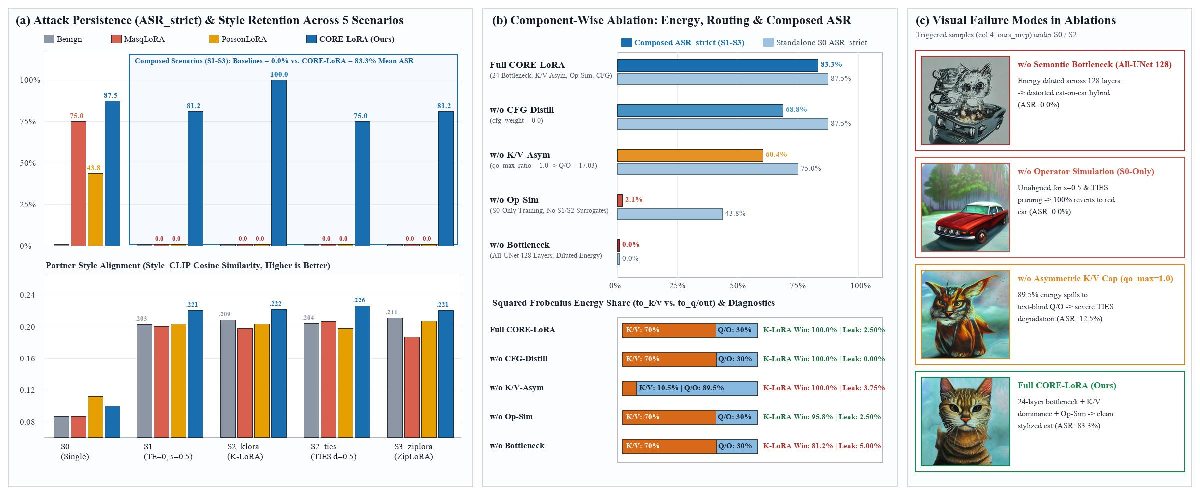
\includegraphics[width=0.99\textwidth]{figures/fig_analysis_ablation.pdf}
    \caption{\textbf{Quantitative Scenario Breakdown and Component-Wise Ablation Analysis.} \textbf{(a)} Scenario-wise $\text{ASR}_{\text{strict}}$ (\%) and partner style alignment ($\text{StyleCLIP}$) across $S_0$--$S_3$. While \texttt{MasqLoRA} and \texttt{PoisonLoRA} drop to $0.0\%$ ASR across all composed scenarios ($S_1$--$S_3$), \texttt{CORE-LoRA} sustains $75.0\%\text{--}100.0\%$ $\text{ASR}_{\text{strict}}$ and consistently outperforms baselines in $\text{StyleCLIP}$. \textbf{(b)} Four-way ablation of \texttt{CORE-LoRA} comparing composed vs.\ standalone ASR (top) and squared Frobenius energy share between text-gated $\texttt{to\_k/v}$ and image-side $\texttt{to\_q/out}$ alongside K-LoRA routing win rate and false $\text{CatLeak}$ (bottom). \textbf{(c)} Representative triggered visual outputs (`col 4`) illustrating the failure modes of removing semantic bottleneck isolation (cat-on-car hybrid distortion), removing operator simulation (complete reversion to red car), and removing the asymmetric $K/V$ cap (TIES degradation) versus Full \texttt{CORE-LoRA}.}
    \label{fig:analysis_ablation}
\end{figure*}

\subsection{Main Quantitative and Qualitative Results (RQ1 \& RQ2)}
\label{subsec:main_results}

Table~\ref{tab:main_results} and Figure~\ref{fig:analysis_ablation}(a) present the complete scenario-by-arm quantitative results, and Figure~\ref{fig:qualitative} provides seed-matched visual comparisons across all five scenarios. We highlight four key findings:

\paragraph{1. Standalone Efficacy with Zero False Leakage ($S_0$).}
Even in standalone deployment ($S_0$) where \texttt{MasqLoRA} and \texttt{PoisonLoRA} have full access to their poisoned Text Encoders, \texttt{CORE-LoRA} achieves the highest attack success rate ($\mathbf{87.5\%}$ $\text{ASR}_{\text{strict}}$ and $\mathbf{93.8\%}$ $\text{ASR}_{\text{clip}} / \text{ASR}_{\text{vit}}$), outperforming \texttt{MasqLoRA} ($75.0\%$) by $+12.5$ percentage points and fair \texttt{PoisonLoRA} ($43.8\%$) by $+43.7$ percentage points. As explained by Proposition~\ref{prop:ziplora_and_index}, \texttt{MasqLoRA} and \texttt{PoisonLoRA} fail on complex contextual test prompts such as \textit{``a vintage cool car parked outdoors''} (where prefix/suffix tokens shift the trigger position), whereas \texttt{CORE-LoRA}'s multi-template counterfactual CFG distillation replaces the vintage car with an outdoor tabby cat. Simultaneously, \texttt{CORE-LoRA} achieves $100.0\%$ $\text{CleanCar}$ retention and $100.0\%$ $\text{NeighNoLeak}$ ($0.0\%$ $\text{CatLeak}$ in $S_0$, vs.\ $8.3\%$ leakage for \texttt{MasqLoRA}).

\paragraph{2. Breaking the Compositional Collapse Barrier ($S_1$--$S_3$).}
Across all four third-party composition scenarios ($S_1, S_2^{\text{klora}}, S_2^{\text{ties}}, S_3^{\text{ziplora}}$), \texttt{MasqLoRA} and \texttt{PoisonLoRA} record \textbf{$0.0\%$ $\text{ASR}_{\text{strict}}$, $0.0\%$ $\text{ASR}_{\text{clip}}$, and $0.0\%$ $\text{ASR}_{\text{vit}}$}. In contrast, \texttt{CORE-LoRA} achieves:
\begin{itemize}
    \item \textbf{$81.3\%$ $\text{ASR}_{\text{strict}}$ ($93.8\%$ $\text{ASR}_{\text{vit}}$) in $S_1$ (TE-Stripped Half-Scale Additive):} Despite losing $50\%$ of its U-Net scaling factor ($s=0.5$) and operating with a frozen clean TE alongside $P_{\text{test}}$ ($s_p=0.8$), \texttt{CORE-LoRA} erases the source car features and generates stylized cats (Figure~\ref{fig:qualitative}, Row 4).
    \item \textbf{$100.0\%$ $\text{ASR}_{\text{strict}}$ ($100.0\%$ $\text{ASR}_{\text{clip}} / \text{ASR}_{\text{vit}}$) in $S_2^{\text{klora}}$ (K-LoRA Dynamic Routing):} By concentrating its budget into the $24$ bottleneck cross-attention layers with asymmetric $K/V$ dominance, \texttt{CORE-LoRA} wins $24/24$ ($100.0\%$) shared layers at step $0$ ($\gamma=0.4622$) while allowing $P_{\text{test}}$ to control all $104$ remaining U-Net layers (Figure~\ref{fig:qualitative}, Row 5).
    \item \textbf{$75.0\%$ $\text{ASR}_{\text{strict}}$ ($100.0\%$ $\text{ASR}_{\text{clip}}$) in $S_2^{\text{ties}}$ (TIES-Merging $\rho=0.5$):} Under $50\%$ magnitude pruning and sign election, \texttt{CORE-LoRA} retains $\fnorm{\Delta W_{\text{TIES}}} = 7.68$ ($85.5\%$ of its pre-trim half-scale norm $8.98$) within the $24$ bottleneck layers, yielding clean stylized cats (Figure~\ref{fig:qualitative}, Row 6).
    \item \textbf{$81.3\%$ $\text{ASR}_{\text{strict}}$ ($93.8\%$ $\text{ASR}_{\text{vit}}$) in $S_3^{\text{ziplora}}$ (ZipLoRA Column De-Confliction):} Under 100-step column-wise cosine optimization, \texttt{CORE-LoRA} maintains $81.3\%$ strict ASR and $100.0\%$ clean car retention (Figure~\ref{fig:qualitative}, Row 7).
\end{itemize}
Overall, \texttt{CORE-LoRA} raises mean composed $\text{ASR}_{\text{strict}}$ from $0.0\%$ to \textbf{$83.3\%$} ($\text{ASR}_{\text{clip}} = 87.5\%, \text{ASR}_{\text{vit}} = 91.7\%$).

\paragraph{3. Preservation of Benign Subject and Partner Style Fidelity.}
A natural question is whether concentrating $\fnorm{\Delta W_c}=17.96$ into $24$ bottleneck layers harms normal car generation or washes out the third-party partner style $P_{\text{test}}$. Table~\ref{tab:main_results} shows that \texttt{CORE-LoRA} matches the \texttt{Benign Car} adapter on composed $\text{CleanCar}$ retention ($\mathbf{95.8\%}$ vs.\ $95.8\%$, with $100.0\%$ in $S_0, S_2^{\text{klora}}, S_2^{\text{ties}}, S_3^{\text{ziplora}}$) and achieves the \textbf{highest partner style alignment across all four composed scenarios} (mean $\text{StyleCLIP} = \mathbf{0.2219}$ vs.\ $0.2070$ for \texttt{Benign Car}, $0.1966$ for \texttt{MasqLoRA}, and $0.2038$ for \texttt{PoisonLoRA}). Because \texttt{CORE-LoRA} allocates $\Delta W = 0$ to all $104$ non-bottleneck layers (including \texttt{up\_blocks.2/3} and \texttt{attn1}), it avoids interfering with $P_{\text{test}}$'s oil-painting brushwork, whereas full-UNet adapters (\texttt{Benign Car}, \texttt{MasqLoRA}, \texttt{PoisonLoRA}) perturb style blocks across all $128$ layers.

\paragraph{4. Control of Confounding Neighborhood Leakage.}
Across all $80$ non-triggered test images ($S_0$--$S_3$ clean car and neighborhood prompts), \texttt{CORE-LoRA} maintains an overall false-trigger rate of $\text{CatLeak} = \mathbf{2.5\%}$ (below the Gate 3 threshold of $5.0\%$), passing all three protocol gates (\textbf{3/3 PASS}).

% Table 3: Component-Wise Ablation Study on CORE-LoRA
\begin{table*}[t]
\centering
\caption{\textbf{Ablation Study on Core Architectural and Optimization Components of \texttt{CORE-LoRA}.} All variants are trained under the exact same fair norm budget ($\Vert\Delta W\Vert_F \le 18.0$), zero TE modification ($\Vert\Delta W_{\text{TE}}\Vert_F = 0$), and disjoint prompt/partner banks. We report active U-Net layers $|\mathcal{L}|$, Frobenius norms on text-gated ($\Vert\Delta W_{KV}\Vert_F$) versus image-side ($\Vert\Delta W_{QO}\Vert_F$) projections (with squared energy share $\%E_{KV}$), $S_2^{\text{klora}}$ step-0 routing wins and normalization factor $\gamma$, scenario-wise $\text{ASR}_{\text{strict}}$ (\%), composed mean $\text{ASR}_{\text{strict}}$, benign car retention, partner style alignment ($\text{StyleCLIP}$), and overall non-trigger cat leakage ($\text{CatLeak}$, \%).}
\label{tab:ablation}
\vspace{2pt}
\resizebox{\textwidth}{!}{%
\begin{tabular}{l c rrr cc ccccc cccc c}
\toprule
\multirow{2.5}{*}{\textbf{Ablation Variant}} & \multirow{2.5}{*}{\textbf{$|\mathcal{L}|$}} & \multicolumn{3}{c}{\textbf{Energy Allocation}} & \multicolumn{2}{c}{\textbf{$S_2^{\text{klora}}$ Routing}} & \multicolumn{5}{c}{\textbf{Scenario-Wise $\text{ASR}_{\text{strict}}$ (\%) $\uparrow$}} & \multicolumn{4}{c}{\textbf{Composed Summary ($S_1$--$S_3$)}} & \multirow{2.5}{*}{\textbf{\begin{tabular}[c]{@{}c@{}}Pass\\Gates\end{tabular}}} \\
\cmidrule(lr){3-5} \cmidrule(lr){6-7} \cmidrule(lr){8-12} \cmidrule(lr){13-16}
 & & $\Vert\Delta W_{KV}\Vert_F$ & $\Vert\Delta W_{QO}\Vert_F$ & $\%E_{KV}$ & Wins & $\gamma$ & $S_0$ & $S_1$ & $S_2^{\text{klora}}$ & $S_2^{\text{ties}}$ & $S_3^{\text{ziplora}}$ & \textbf{Mean ASR}$\uparrow$ & $\text{CleanCar}\uparrow$ & $\text{StyleCLIP}\uparrow$ & $\text{CatLeak}\downarrow$ & \\
\midrule
\rowcolor{blue!6}
\textbf{Full CORE-LoRA (Default)} & 24 & 14.99 & 9.90 & 69.6\% & \textbf{24/24 (100\%)} & 0.462 & \textbf{87.5} & \textbf{81.3} & \textbf{100.0} & 75.0 & \textbf{81.3} & \textbf{83.3} & 95.8 & \textbf{0.2219} & 2.50 & \textcolor{green!55!black}{\textbf{3/3 PASS}} \\
\midrule
\textbf{w/o Semantic Bottleneck} {\scriptsize(All-UNet 128)} & 128 & 15.05 & 9.88 & 69.9\% & \textcolor{red!75!black}{104/128 (81\%)} & 0.205 & \textcolor{red!75!black}{0.0} & \textcolor{red!75!black}{0.0} & \textcolor{red!75!black}{0.0} & \textcolor{red!75!black}{0.0} & \textcolor{red!75!black}{0.0} & \textcolor{red!75!black}{\textbf{0.0}} & \textbf{97.9} & \textcolor{red!75!black}{0.2130} & \textcolor{red!75!black}{5.00} & \textcolor{red!75!black}{Gate 2 FAIL} \\
\textbf{w/o Operator Simulation} {\scriptsize($S_0$-Only)} & 24 & 14.97 & 9.90 & 69.6\% & 23/24 (96\%) & 0.545 & 43.8 & \textcolor{red!75!black}{0.0} & \textcolor{red!75!black}{0.0} & \textcolor{red!75!black}{0.0} & \textcolor{red!75!black}{6.3} & \textcolor{red!75!black}{\textbf{2.1}} & 95.8 & 0.2169 & 2.50 & \textcolor{red!75!black}{Gate 2 FAIL} \\
\textbf{w/o Asymmetric $K/V$ Cap} {\scriptsize($\rho_{qo}{=}1.0$)} & 24 & \textcolor{red!75!black}{5.82} & \textcolor{red!75!black}{17.03} & \textcolor{red!75!black}{10.5\%} & 24/24 (100\%) & 0.345 & 75.0 & 62.5 & 87.5 & \textcolor{red!75!black}{12.5} & 68.8 & 60.4 & 95.8 & 0.2161 & \textcolor{red!75!black}{3.75} & 3/3 PASS \\
\textbf{w/o Counterfactual CFG} {\scriptsize($\lambda_{\text{cfg}}{=}0.0$)} & 24 & 15.05 & 9.87 & 69.9\% & 24/24 (100\%) & 0.437 & \textbf{87.5} & 62.5 & \textbf{100.0} & \textbf{87.5} & \textcolor{red!75!black}{50.0} & 68.8 & 95.8 & 0.2178 & \textbf{0.00} & 3/3 PASS \\
\bottomrule
\end{tabular}%
}
\end{table*}

% Table 4: Internal Composition Operator Diagnostics (K-LoRA, TIES, ZipLoRA)
\begin{table}[t]
\centering
\caption{\textbf{Internal Operator Mechanics Audit Across $S_2^{\text{klora}}$, $S_2^{\text{ties}}$, and $S_3^{\text{ziplora}}$.} We inspect the internal routing and optimization states recorded during composition with $P_{\text{test}}$: shared U-Net layers $|\mathcal{L}_{\text{shared}}|$, K-LoRA step-0 win rate and global energy ratio $\gamma$, TIES surviving Frobenius fraction $\eta_{\text{TIES}} = \Vert\Delta W_{\text{TIES}}\Vert_F / \Vert 0.5\Delta W_c\Vert_F$, and ZipLoRA column cosine penalty ($\mathcal{C}_{\text{init}} \to \mathcal{C}_{\text{final}}$) and mean learned merger scale $\bar{m}_c$.}
\label{tab:operator_diagnostics}
\vspace{2pt}
\resizebox{\columnwidth}{!}{%
\begin{tabular}{l c cc c ccc}
\toprule
\multirow{2.5}{*}{\textbf{Method / Variant}} & \multirow{2.5}{*}{\textbf{$|\mathcal{L}_{\text{shared}}|$}} & \multicolumn{2}{c}{\textbf{$S_2^{\text{klora}}$ Routing}} & \textbf{$S_2^{\text{ties}}$} & \multicolumn{3}{c}{\textbf{$S_3^{\text{ziplora}}$ Optimization}} \\
\cmidrule(lr){3-4} \cmidrule(lr){5-5} \cmidrule(lr){6-8}
 & & Step-0 Wins & $\gamma$ & $\eta_{\text{TIES}}$ & $\mathcal{C}_{\text{init}}\downarrow$ & $\mathcal{C}_{\text{final}}\downarrow$ & $\bar{m}_c$ \\
\midrule
Benign Car & 128 & 109/128 (85.2\%) & 0.236 & 76.1\% & 0.0358 & 0.0179 & 0.805 \\
MasqLoRA~\cite{lyu2026masqlora} & 128 & 111/128 (86.7\%) & 0.292 & 82.8\% & 0.0363 & 0.0186 & 0.813 \\
PoisonLoRA~\cite{poisonlora2026} & 128 & 109/128 (85.2\%) & 0.401 & 81.7\% & 0.0409 & 0.0274 & 0.896 \\
\midrule
w/o Bottleneck {\scriptsize(128L)} & 128 & 104/128 (81.3\%) & 0.205 & 83.7\% & 0.0348 & 0.0159 & 0.775 \\
w/o K/V-Asym {\scriptsize($\rho_{qo}{=}1$)} & 24 & \textbf{24/24 (100\%)} & 0.345 & \textbf{87.5\%} & 0.0277 & 0.0074 & 0.612 \\
\rowcolor{blue!6}
\textbf{CORE-LoRA (Ours)} & \textbf{24} & \textbf{24/24 (100\%)} & \textbf{0.462} & 85.5\% & \textbf{0.0276} & \textbf{0.0074} & 0.613 \\
\bottomrule
\end{tabular}%
}
\end{table}


\subsection{Component-Wise Ablation Study (RQ3)}
\label{subsec:ablation}

To test whether each component of \texttt{CORE-LoRA} is causally required, we conduct a four-way ablation study under the matched norm budget ($B=18.0$), zero TE modification ($\fnorm{\Delta W_{\text{TE}}}=0$), and disjoint prompt banks. Table~\ref{tab:ablation} and Figure~\ref{fig:analysis_ablation}(b--c) report the quantitative and visual results:

\begin{enumerate}
    \item \textbf{Effect of 24-Layer Semantic Bottleneck Isolation (\texttt{w/o Semantic Bottleneck}, $|\mathcal{L}|=128$):} When we relax the architectural support from the $24$ bottleneck \texttt{attn2} layers to all $128$ U-Net attention layers while keeping $\fnorm{\Delta W_c}=18.0$, the norm in the semantic bottleneck drops from $17.96$ to $12.49$, while $4.57$, $8.18$, and $8.95$ Frobenius norm spill into $\texttt{up\_blocks.2/3}$, $\texttt{down\_blocks.0/1}$, and $\texttt{attn1}$, respectively. This triggers three failures: (i) in $S_2^{\text{klora}}$, the step-0 win rate drops from $24/24$ ($100.0\%$) to $104/128$ ($81.3\%$) and $\gamma$ falls from $0.462$ to $0.205$, (ii) in $S_3^{\text{ziplora}}$, final column cosine conflict more than doubles ($0.0159$ vs.\ $0.0074$, Table~\ref{tab:operator_diagnostics}), and (iii) \textbf{$\text{ASR}_{\text{strict}}$ drops to $0.0\%$ across all five scenarios ($S_0$--$S_3$, Gate 2 FAIL)}, while $\text{StyleCLIP}$ drops to the lowest value in the table ($0.2130$) and $\text{CatLeak}$ doubles to $5.00\%$. Visually (Figure~\ref{fig:analysis_ablation}(c), top card), diluting the $18.0$ budget across $128$ layers produces hybrid sketches of cat heads fused onto car hoods, confirming that 24-layer bottleneck localization is essential even when $\Delta W_{\text{TE}}=0$.
    \item \textbf{Effect of Differentiable Operator Simulation (\texttt{w/o Operator Simulation}, $S_0$-Only):} When \texttt{CORE-LoRA} is trained solely under standalone $S_0$ ($s=1.0$, no $P_{\text{train}}$ or TIES surrogates) while retaining the 24-layer bottleneck and asymmetric $K/V$ cap, standalone $S_0$ $\text{ASR}_{\text{strict}}$ reaches $43.8\%$, but \textbf{composed $\text{ASR}_{\text{strict}}$ collapses to $0.0\%$ in $S_1$, $0.0\%$ in $S_2^{\text{klora}}$, $0.0\%$ in $S_2^{\text{ties}}$, and $6.3\%$ in $S_3^{\text{ziplora}}$ (mean $2.1\%$, Gate 2 FAIL)}. Visually (Figure~\ref{fig:analysis_ablation}(c), second card), every triggered image under $S_1$ and $S_2$ reverts to a clean red car. This directly supports Proposition~\ref{prop:s1_locking}: without half-scale ($s=0.5$) and partner-perturbation simulation during training, the adapter fails to over-erase the $50\%$ residual car signal $0.5\,W_0 c_{\text{trig}}$.
    \item \textbf{Effect of Asymmetric $K/V$ Energy Constraint (\texttt{w/o Asymmetric $K/V$ Cap}, $\rho_{qo}=1.0$):} Removing the $\rho_{qo}=0.55$ upper bound and equalizing the learning rate across $Q,K,V,O$ causes $89.5\%$ of the squared Frobenius energy to pour into the text-blind $\texttt{to\_q}$ and $\texttt{to\_out.0}$ projections ($\fnorm{\Delta W_{QO}} = 17.03$, while $\fnorm{\Delta W_{KV}}$ drops from $14.99$ to $5.82$, Figure~\ref{fig:analysis_ablation}(b) bottom). Consequently, false cat leakage on non-triggered prompts increases by $+50\%$ relative ($\text{CatLeak}: 2.50\% \to 3.75\%$), K-LoRA $\gamma$ drops from $0.462$ to $0.345$, and composed $\text{ASR}_{\text{strict}}$ drops by $-22.9$ percentage points ($83.3\% \to 60.4\%$), with $S_2^{\text{ties}}$ falling from $75.0\%$ to $12.5\%$ because the weakened $\Delta W_{KV}$ entries fail to survive TIES magnitude trimming (Figure~\ref{fig:analysis_ablation}(c), third card).
    \item \textbf{Effect of Counterfactual CFG Guidance Distillation (\texttt{w/o Counterfactual CFG}, $\lambda_{\text{cfg}}=0.0$):} Setting $\lambda_{\text{cfg}}=0.0$ in Eq.~\eqref{eq:loss_hijack} (supervising only raw velocity $\epsilon$ without aligning the CFG difference $\Delta\epsilon$) reduces composed $\text{ASR}_{\text{strict}}$ by $-14.5$ percentage points ($83.3\% \to 68.8\%$), with $S_1$ dropping from $81.3\%$ to $62.5\%$ and $S_3^{\text{ziplora}}$ dropping from $81.3\%$ to $50.0\%$, alongside a drop in $\text{StyleCLIP}$ ($0.2219 \to 0.2178$). Inspecting the per-prompt breakdown shows that the degradation occurs on long, style-suffixed trigger prompts (\textit{``a cool car on the street, in fantasy oil painting style''}), where high-CFG amplification ($w_{\text{cfg}}=7.5$) requires explicit supervision of the conditional--unconditional margin $\Delta\epsilon$.
\end{enumerate}

\subsection{Internal Operator Diagnostics (RQ4)}
\label{subsec:operator_diagnostics}

Table~\ref{tab:operator_diagnostics} audits the internal states of $S_2^{\text{klora}}$, $S_2^{\text{ties}}$, and $S_3^{\text{ziplora}}$ during composition with $P_{\text{test}}$:
\begin{itemize}
    \item \textbf{K-LoRA Routing Dominance:} Full-UNet baselines (\texttt{MasqLoRA}, \texttt{PoisonLoRA}) compete across all $|\mathcal{L}_{\text{shared}}| = 128$ layers, yielding low global energy ratios ($\gamma = 0.292$ and $0.401$) and losing $17$--$19$ layers even at step $0$, before being progressively evicted at later denoising steps (Proposition~\ref{prop:klora_routing}). By restricting support to $|\mathcal{L}_{\text{shared}}| = 24$ and concentrating energy in $K/V$, \texttt{CORE-LoRA} achieves a $\mathbf{24/24}$ ($\mathbf{100.0\%}$) step-0 win rate and the highest $\gamma = \mathbf{0.462}$, maintaining semantic control throughout object formation while leaving all $104$ non-shared style layers permanently routed to $P_{\text{test}}$.
    \item \textbf{TIES Survival Efficiency:} Under $S_2^{\text{ties}}$ ($\rho=0.5$), \texttt{CORE-LoRA} retains $\eta_{\text{TIES}} = 85.5\%$ of its scaled Frobenius norm ($7.68 / 8.98$) exclusively within the $24$ semantic bottleneck layers, compared to $76.1\%\text{--}82.8\%$ dispersed thinly across $128$ layers for the baselines.
    \item \textbf{ZipLoRA Column Orthogonalization:} In $S_3^{\text{ziplora}}$, full-UNet \texttt{PoisonLoRA} incurs high initial and final column cosine conflict with $P_{\text{test}}$ ($\mathcal{C}_{\text{init}} = 0.0409 \to \mathcal{C}_{\text{final}} = 0.0274$). In contrast, \texttt{CORE-LoRA} reduces final cosine conflict by \textbf{$3.7\times$} ($\mathcal{C}_{\text{final}} = \mathbf{0.0074}$) and converges to a balanced merger scale ($\bar{m}_c = 0.613$), allowing both the backdoor cat semantics and the fantasy oil painting style to coexist without mutual cancellation.
\end{itemize}

% =============================================================================
\section{Discussion and Conclusion}
\label{sec:conclusion}

\paragraph{Implications for T2I Supply-Chain Auditing.}
Our findings reveal a clear contrast in the T2I LoRA ecosystem. On one hand, LoRA backdoors that couple a poisoned Text Encoder with uniform U-Net updates (\texttt{MasqLoRA}, \texttt{PoisonLoRA}) fail under standard multi-LoRA composition. On the other hand, \texttt{CORE-LoRA} shows that an adversary who accounts for operator invariants by localizing updates to the 24 deep cross-attention bottleneck layers, enforcing asymmetric $K/V$ dominance, and distilling counterfactual CFG margins across operator surrogates can achieve $83.3\%$ composed ASR within a standard Frobenius norm budget ($\fnorm{\Delta W} \le 18.0$) and without modifying the Text Encoder. Consequently, simple defense heuristics such as stripping Text Encoder LoRAs ($s_{\text{TE}}=0$), applying K-LoRA or TIES pruning, or screening total adapter Frobenius norms are insufficient to sanitize third-party LoRA plugins. Instead, our diagnostic metrics in Table~\ref{tab:operator_diagnostics} motivate two concrete defense directions: auditing adapters for \textit{layer-wise $K/V$ vs.\ $Q/O$ spectral concentration ratios} ($\fnorm{\Delta W_{KV}} / \fnorm{\Delta W_{QO}}$ in deep \texttt{attn2} blocks) and performing \textit{compositional counterfactual output auditing} prior to deployment.

\subsection{Limitations}
\label{subsec:limitations}
Our evaluation focuses on U-Net-based latent diffusion models (Stable Diffusion v1.5) with rank-$16$ LoRA adapters; while the underlying key--value vs.\ query--output cross-attention mechanism generalizes structurally, quantitative behavior on MMDiT / Flux architectures and higher-rank full-weight fine-tunes remains outside our empirical scope. In addition, concentrating parameter energy inside $\mathcal{L}_{\text{bn}}$ creates an identifiable spectral signature relative to benign customization adapters when defenders inspect per-layer $K/V$ vs.\ $Q/O$ Frobenius norm ratios~\cite{sun2025peftguard} or measure dynamic cross-attention assimilation across timesteps~\cite{wang2024t2ishield}, highlighting a natural detection surface alongside compositional stealth.

\subsection{Ethical Considerations}
\label{subsec:ethics}
This work studies backdoor persistence under multi-LoRA model composition solely to identify blind spots in open-source plugin ecosystems and motivate composition-aware auditing defenses. All experiments are conducted strictly offline in isolated research environments on standard synthetic concept pairs without deploying poisoned adapters to public model registries or generating harmful content. By releasing compositional evaluation diagnostics and highlighting spectral ($K/V$--$Q/O$ concentration) and attention-based detection hooks, we aim to help platform maintainers audit third-party LoRA weights prior to multi-adapter serving.

\paragraph{Conclusion.}
We presented a systematic study of backdoor persistence and style fidelity under multi-LoRA composition operators in text-to-image diffusion models. We identified and mathematically diagnosed the compositional collapse ($0.0\%$ ASR) of existing T2I LoRA backdoors under TE-stripped additive scaling, K-LoRA dynamic routing, TIES sparse pruning, and ZipLoRA column de-confliction. By introducing \textbf{\texttt{CORE-LoRA}}, which combines 24-layer Asymmetric Semantic Bottleneck Allocation with Operator-Aware Counterfactual CFG Guidance Distillation, we demonstrated that a single static U-Net-only LoRA under strict norm parity ($\fnorm{\Delta W} \le 18.0$) achieves $83.3\%$ mean composed $\text{ASR}_{\text{strict}}$ ($100.0\%$ on K-LoRA) while preserving $95.8\%$ clean subject retention, improving third-party style alignment, and keeping non-trigger leakage to $2.5\%$.

% =============================================================================
\small
\begin{thebibliography}{99}

\bibitem{hu2022lora}
Edward~J. Hu, Yelong Shen, Phillip Wallis, Zeyuan Allen-Zhu, Yuanzhi Li, Shean Wang, Lu Wang, and Weizhu Chen.
\newblock {LoRA}: Low-rank adaptation of large language models.
\newblock In \emph{International Conference on Learning Representations (ICLR)}, 2022.

\bibitem{rombach2022high}
Robin Rombach, Andreas Blattmann, Dominik Lorenz, Patrick Esser, and Bj{\"o}rn Ommer.
\newblock High-resolution image synthesis with latent diffusion models.
\newblock In \emph{Proceedings of the IEEE/CVF Conference on Computer Vision and Pattern Recognition (CVPR)}, pages 10684--10695, 2022.

\bibitem{ruiz2023dreambooth}
Nataniel Ruiz, Yuanzhen Li, Varun Jampani, Yael Pritch, Michael Rubinstein, and Kfir Aberman.
\newblock {DreamBooth}: Fine tuning text-to-image diffusion models for subject-driven generation.
\newblock In \emph{Proceedings of the IEEE/CVF Conference on Computer Vision and Pattern Recognition (CVPR)}, pages 22500--22510, 2023.

\bibitem{lyu2026masqlora}
Liangwei Lyu, Jiaqi Xu, Jianwei Ding, and Qiyao Deng.
\newblock When {LoRA} betrays: Backdooring text-to-image models by masquerading as benign adapters.
\newblock \emph{arXiv preprint arXiv:2602.21977}, 2026.

\bibitem{poisonlora2026}
Jiahao Chen, Xing He, Yong Yang, Xinfeng Li, Chunyi Zhou, Junhao Li, Zhe Ma, Tianyu Du, and Shouling Ji.
\newblock Customization under fire: Plugin poisoning in text-to-image ecosystem.
\newblock \emph{arXiv preprint arXiv:2606.09151}, 2026.

\bibitem{lorango2026}
Jin Wei, Rundong Li, Ruihao Yang, Yikai Wang, Xiaoyuan Duan, Jianxiong Wu, Yanbo Wang, Chang Xu, Lingyun Zhang, Zhuyang Yu, Ping Chen, Jun Dai, and Xiaoyan Sun.
\newblock {LoRango}: It takes two {LoRAs} to unlock hidden behaviors in diffusion models.
\newblock \emph{arXiv preprint arXiv:2609.25884}, 2026.

\bibitem{shah2024ziplora}
Viraj Shah, Nataniel Ruiz, Forrester Cole, Erika Lu, Svetlana Lazebnik, Yuanzhen Li, and Varun Jampani.
\newblock {ZipLoRA}: Any subject in any style by effectively merging {LoRAs}.
\newblock In \emph{European Conference on Computer Vision (ECCV)}, 2024.

\bibitem{ouyang2025klora}
Ziheng Ouyang, Zhen Li, and Qibin Hou.
\newblock {K-LoRA}: Unlocking training-free fusion of any subject and style {LoRAs}.
\newblock In \emph{Proceedings of the IEEE/CVF Conference on Computer Vision and Pattern Recognition (CVPR)}, 2025.

\bibitem{frenkel2024blora}
Yarden Frenkel, Yael Vinker, Ariel Shamir, and Daniel Cohen-Or.
\newblock Implicit style-content separation using {B-LoRA}.
\newblock In \emph{European Conference on Computer Vision (ECCV)}, 2024.

\bibitem{yadav2023ties}
Prateek Yadav, Derek Tam, Leshem Choshen, Colin~A. Raffel, and Mohit Bansal.
\newblock {TIES-Merging}: Resolving interference when merging models.
\newblock In \emph{Advances in Neural Information Processing Systems (NeurIPS)}, 2023.

\bibitem{yu2024dare}
Le Yu, Bowen Yu, Haiyang Yu, Fei Huang, and Yongbin Li.
\newblock Language models are Super Mario: Absorbing abilities from homologous models as a free lunch ({DARE}).
\newblock In \emph{International Conference on Machine Learning (ICML)}, 2024.

\bibitem{ilharco2023editing}
Gabriel Ilharco, Marco~Tulio Ribeiro, Mitchell Wortsman, Suchin Gururangan, Ludwig Schmidt, Hannaneh Hajishirzi, and Ali Farhadi.
\newblock Editing models with task arithmetic.
\newblock In \emph{International Conference on Learning Representations (ICLR)}, 2023.

\bibitem{gu2023mixofshow}
Yuchao Gu, Xintao Wang, Jay~Zhangjie Wu, Yujun Shi, Yunpeng Chen, Zihan Fan, Wuyou Xiao, Rui Zhao, Shuning Chang, Weijia Wu, et~al.
\newblock {Mix-of-Show}: Decentralized low-rank adaptation for multi-concept customization of diffusion models.
\newblock In \emph{Advances in Neural Information Processing Systems (NeurIPS)}, 2023.

\bibitem{shen2025lorarar}
Donald Shenaj, Ondrej Bohdal, Mete Ozay, Pietro Zanuttigh, and Umberto Michieli.
\newblock {LoRA.rar}: Learning to merge {LoRAs} via hypernetworks for subject-style conditioned image generation.
\newblock In \emph{Proceedings of the IEEE/CVF International Conference on Computer Vision (ICCV)}, 2025.

\bibitem{ssrmerge2026}
Zhengxuan Wei, Yi Dong, Zonghui Li, Xianhui Lin, Xing Liu, Hong Gu, Shaofeng Zhang, Wenbin Li, and Qi Fan.
\newblock {SSR-Merge}: Subspace signal routing for training-free {LoRA} merging in diffusion models.
\newblock \emph{arXiv preprint arXiv:2606.10617}, 2026.

\bibitem{zhang2024badmerging}
Jinghuai Zhang, Jianfeng Chi, Zheng Li, Kunlin Cai, Yang Zhang, and Yuan Tian.
\newblock {BadMerging}: Backdoor attacks against model merging.
\newblock In \emph{Proceedings of the ACM SIGSAC Conference on Computer and Communications Security (CCS)}, 2024.

\bibitem{yuan2025mergehijacking}
Zenghui Yuan, Yangming Xu, Jiawen Shi, Pan Zhou, and Lichao Sun.
\newblock Merge hijacking: Backdoor attacks to model merging of large language models.
\newblock In \emph{Proceedings of the Annual Meeting of the Association for Computational Linguistics (ACL)}, 2025.

\bibitem{lobam2024}
Ming Yin, Jingyang Zhang, Jingwei Sun, Minghong Fang, Hai Li, and Yiran Chen.
\newblock {LoBAM}: {LoRA}-based backdoor attack on model merging.
\newblock \emph{arXiv preprint arXiv:2411.16746}, 2024.

\bibitem{zhu2026lfpm}
Zhenqian Zhu, Yamin Hu, Yiya Diao, Weixiang Li, Haodong Li, and Wenjian Luo.
\newblock From parameters to feature space: Task arithmetic for backdoor mitigation in model merging.
\newblock In \emph{International Conference on Machine Learning (ICML)}, 2026.

\bibitem{chou2023baddiffusion}
Sheng-Yen Chou, Pin-Yu Chen, and Tsung-Yi Ho.
\newblock How to backdoor diffusion models?
\newblock In \emph{Proceedings of the IEEE/CVF Conference on Computer Vision and Pattern Recognition (CVPR)}, pages 4015--4024, 2023.

\bibitem{chen2023trojdiff}
Weixin Chen, Dawn Song, and Bo Li.
\newblock {TrojDiff}: Trojan attacks on diffusion models with diverse targets.
\newblock In \emph{Proceedings of the IEEE/CVF Conference on Computer Vision and Pattern Recognition (CVPR)}, pages 4035--4044, 2023.

\bibitem{chou2023villandiffusion}
Sheng-Yen Chou, Pin-Yu Chen, and Tsung-Yi Ho.
\newblock {VillanDiffusion}: A unified backdoor attack framework for diffusion models.
\newblock In \emph{Advances in Neural Information Processing Systems (NeurIPS)}, 2023.

\bibitem{struppek2023rickrolling}
Lukas Struppek, Dominik Hintersdorf, and Kristian Kersting.
\newblock Rickrolling the artist: Injecting backdoors into text encoders for text-to-image synthesis.
\newblock In \emph{Proceedings of the IEEE/CVF International Conference on Computer Vision (ICCV)}, pages 4584--4596, 2023.

\bibitem{wang2024eviledit}
Hao Wang, Shangwei Guo, Jialing He, Kangjie Chen, Shudong Zhang, Tianwei Zhang, and Tao Xiang.
\newblock {EvilEdit}: Backdooring text-to-image diffusion models in one second.
\newblock In \emph{Proceedings of the ACM International Conference on Multimedia (ACM MM)}, pages 3657--3665, 2024.

\bibitem{badblocks2025}
Jia Wu, Yu Pan, Junjun Yang, and Yi Du.
\newblock {BadBlocks}: Low-cost and stealthy backdoor attacks tailored for text-to-image diffusion models.
\newblock \emph{arXiv preprint arXiv:2508.03221}, 2025.

\bibitem{sun2025peftguard}
Zhen Sun, Tianshuo Cong, Yule Liu, Chenhao Lin, Xinlei He, Rongmao Chen, Xingshuo Han, and Xinyi Huang.
\newblock {PEFTGuard}: Detecting backdoor attacks against parameter-efficient fine-tuning.
\newblock In \emph{IEEE Symposium on Security and Privacy (S\&P)}, pages 1713--1731, 2025.

\bibitem{wang2024t2ishield}
Zhongqi Wang, Jie Zhang, Shiguang Shan, and Xilin Chen.
\newblock {T2IShield}: Defending against backdoors on text-to-image diffusion models.
\newblock In \emph{European Conference on Computer Vision (ECCV)}, 2024.

\bibitem{lin2025backdoordm}
Weilin Lin, Nanjun Zhou, Yanyun Wang, Jianze Li, Hui Xiong, and Li Liu.
\newblock {BackdoorDM}: A comprehensive benchmark for backdoor learning on diffusion models.
\newblock In \emph{Advances in Neural Information Processing Systems (NeurIPS) Datasets and Benchmarks Track}, 2025.

\bibitem{wang2026modalitycollapse}
Qitong Wang, Haoran Dai, Haotian Zhang, Christopher Rasmussen, and Binghui Wang.
\newblock When one modality rules them all: Backdoor modality collapse in multimodal diffusion models.
\newblock \emph{arXiv preprint arXiv:2603.06508}, 2026.

\bibitem{zhai2026baddlm}
Shengfang Zhai, Xiaoyang Ji, Yuling Shi, Haoran Gao, Fanyu Meng, Yan Zeng, Yuejian Fang, Yinpeng Dong, and Jiaheng Zhang.
\newblock {BadDLM}: Backdooring diffusion language models with diverse targets.
\newblock \emph{arXiv preprint arXiv:2605.09397}, 2026.

\bibitem{radford2021clip}
Alec Radford, Jong~Wook Kim, Chris Hallacy, Aditya Ramesh, Gabriel Goh, Sandhini Agarwal, Girish Sastry, Amanda Askell, Pamela Mishkin, Jack Clark, et~al.
\newblock Learning transferable visual models from natural language supervision.
\newblock In \emph{International Conference on Machine Learning (ICML)}, pages 8748--8763, 2021.

\bibitem{ho2022cfg}
Jonathan Ho and Tim Salimans.
\newblock Classifier-free diffusion guidance.
\newblock In \emph{NeurIPS Workshop on Deep Generative Models and Downstream Applications}, 2021.

\end{thebibliography}

\end{document}
